% Paper 1 -- Fidetype. Draft v3 (revision round 3), 2026-11-12.
% Build:  tectonic -X compile main.tex --outdir build      (see ../README.md)
% Class: generic one-column article for arXiv. To switch to the IOP Journal of Neural
% Engineering template later, replace the preamble block marked "CLASS" and keep sections/*.tex.
\documentclass[11pt,a4paper]{article}

% ---------------------------------------------------------------- CLASS (swap for IOP template)
\usepackage[a4paper,margin=2.5cm]{geometry}
\usepackage[T1]{fontenc}
\usepackage[utf8]{inputenc}
\usepackage{lmodern}
\usepackage{microtype}
% ---------------------------------------------------------------- packages
\usepackage{amsmath,amssymb}
\usepackage{graphicx}
\usepackage{booktabs}
\usepackage{adjustbox}
\usepackage{enumitem}
\usepackage{multirow}
\usepackage{array}
\usepackage{xcolor}
\usepackage{tikz}
\usetikzlibrary{arrows.meta,positioning,shapes.geometric,fit,calc,backgrounds}
\usepackage[font=small,labelfont=bf]{caption}
\usepackage{subcaption}
\usepackage{placeins}
\usepackage{float}
\usepackage{algorithm}
\usepackage{algpseudocode}
\usepackage[numbers,sort&compress]{natbib}
\usepackage[colorlinks=true,linkcolor=blue!50!black,citecolor=blue!50!black,urlcolor=blue!50!black]{hyperref}
\usepackage{url}
\usepackage[capitalise,noabbrev]{cleveref}

\graphicspath{{../figures/}}
\emergencystretch=2em

% ---------------------------------------------------------------- macros
% \todo{...}: visible red marker for missing data or open decisions. Never remove one
% without filling the gap it names. Grep "\todo" to list them.
\newcommand{\todo}[1]{\textcolor{red}{\textbf{[TODO: #1]}}}
\newcommand{\nts}{NeuralTextStream}
\newcommand{\ewpm}{eWPM}
\newcommand{\act}[1]{\textsc{#1}}
\newcommand{\code}[1]{\texttt{#1}}
\newcommand{\ci}[2]{\ensuremath{[#1,\,#2]}}  % math mode: "-0.11" prints a true minus sign

% Title (v3): shortened after review round 3 (25 -> 15 words). It names the claim (risk-controlled commits)
% and no longer suggests three tests of the commit decision. "Fidetype" stays out of the title (open author decision).
\title{When should a neural text-entry decoder commit?\\Risk-controlled commits from a decoder-agnostic trust layer}
\author{\todo{authors, affiliations, e-mail}}
\date{Draft v3 (revision round 3) --- 12 November 2026 --- not for distribution}

\begin{document}
\maketitle

\begin{abstract}
\noindent\textit{Objective.} Neural text-entry decoders increasingly end in a language model that turns weak neural evidence into fluent sentences, but they rarely signal when a sentence is wrong. We ask when such a system should commit a sentence, offer alternatives or abstain, and whether one decision rule can serve decoders for different recording modalities.
\textit{Approach.} We define an open per-frame output format (\nts{}) and a trust layer that reads only this stream. The layer calibrates confidence, chooses between commit, offer and abstain, and sets its commit threshold with conformal risk control (an expected-risk bound under exchangeability), Learn-then-Test (a high-probability bound) or adaptive online updates from user corrections (a long-run bound). We re-fit the same implementation offline on public data from one intracortical speech participant (816 test trials), forearm surface EMG key presses composed into sentences (19 participants) and MEG typing (19 participants). A simulated eye-gaze user scores each policy in effective words per minute (\ewpm{}) against always committing, always offering and gaze typing alone.
\textit{Main results.} On intracortical speech, the layer cut wrong commits from 61\% to 6\% of sentences at the speed of always committing (11.55 vs 11.45 \ewpm{}) and 1.6\% faster than always offering, but one committed sentence in four was still wrong. As a gate on the published decoder, it cut wrong commits from 19\% to 4\% at a 4.3\% speed cost. On EMG it committed at most 4\% of sentences. On MEG it never committed, and speed did not differ detectably from gaze typing. Conformal calibration held the mean wrong-commit rate at 0.048 (target 0.05) over random splits; online re-calibration kept it at 0.040--0.053 where a threshold fixed on earlier data reached 0.0625--0.0635 \todo{R1: re-check after the clean-calibration drift baseline}. The layer committed no text from signal-destroying control streams, but it cannot detect a real stream of a different intended sentence.
\textit{Significance.} A stream-level commit rule with stated guarantees can make language-model-assisted neural text entry safer without slowing it when the decoder is accurate enough. All speed results are simulations and need a user study.
\end{abstract}

\section{Introduction}
\label{sec:intro}

Brain--computer interfaces (BCIs) for text entry are moving from the laboratory towards products. Intracortical speech neuroprostheses decode attempted speech at conversational rates \citep{willett2023speech,card2024accurate}; handwriting and typing neuroprostheses reach similar speeds \citep{willett2021handwriting,jude2026bimanual}; non-invasive decoders now reconstruct typed sentences from MEG \citep{levy2026brain2qwerty,zhang2026brain2qwertyv2}; and wrist or forearm surface EMG (sEMG) is a candidate input for consumer devices \citep{sivakumar2024emg2qwerty,achituve2025emg}. Most of these systems end in a language-model (LM) stage that turns noisy per-frame predictions into fluent sentences. This stage improves the error rate, but it also makes wrong output look right: a fluent wrong sentence is harder to notice than a garbled one, as known from automatic speech recognition \citep{koenecke2024careless}. For a user who depends on the interface to communicate, a wrong sentence that is committed and sent costs more than a slow one.

Three gaps stand between current decoders and safe use.

\paragraph{No common format for decoder output with honest confidence.} Each decoder reports its output in its own way. The Apple BCI Human Interface Device (HID) profile sends discrete events with a 0--255 ``neural activity strength'' that is not a probability \citep{applebcihid}. W3C EMMA can carry a confidence and an n-best list, but it has no per-frame distributions \citep{w3cemma2009}. Lab Streaming Layer and BIDS move or store raw signals, not decoded text \citep{kothe2024lsl}. A downstream component that wants to decide whether to trust a decoder must therefore be rebuilt for every device.

\paragraph{No decoder-agnostic rule for \emph{when to commit}, with a guarantee.} Calibration \citep{guo2017calibration} and selective prediction \citep{geifman2017selective} are well studied, and recent BCI work adds confidence estimates to single decoders \citep{kim2025confidence}. We know of no layer that works across device types, decides between committing, offering alternatives and abstaining, and states a finite-sample bound on how often it commits wrong text. \todo{G10: add and position the closest work (Huang et al.\ 2025, co-control BCI; Damri \& Laufer-Goldshtein 2026, risk-controlled generative ASR) after their source pages exist.}

\paragraph{Error rates do not show whether a BCI saves the user time.} Character and word error rates (CER, WER) compare decoders, but they do not say whether a user would type faster with the BCI than without it. A no-BCI baseline, such as gaze typing for people with ALS \citep{cai2024gaze}, is rarely reported next to the decoder.

\paragraph{This work.} We address the three gaps with one format, one layer and one evaluation protocol, and we test them on three device types with public data (\cref{fig:arch}). Our contributions are:
\begin{enumerate}
  \item \textbf{A vendor-neutral stream format} (\nts{} v0.1) for neural decoder output: per-frame log-probabilities over a declared vocabulary (characters, keys, phonemes), with timing, calibration and provenance conventions, a conformance suite of 60 checks and 52 golden test vectors, and adapters for MEG, intracortical and sEMG decoders. No breaking change was needed across the three device types (\cref{sec:format}).
  \item \textbf{A decoder-agnostic trust layer} that reads only \nts{}: temperature calibration, a neural-evidence guard, and a \act{commit}/\act{offer}/\act{abstain} policy fitted for maximum \ewpm{} under a wrong-commit limit. It also works as a gate on a black-box, LM-rescored decoder (\cref{sec:trust}).
  \item \textbf{Finite-sample and drift-robust wrong-commit control}: conformal risk control (CRC) and Learn-then-Test (LTT) for the commit threshold \citep{angelopoulos2024crc,angelopoulos2021ltt}, and an online controller that re-calibrates from user feedback, with a long-run bound that holds for any sequence of items for two of its variants \citep{gibbs2021aci,feldman2023rolling}.
  \item \textbf{A privacy-preserving provenance ledger}: an append-only, SHA-256 hash-chained record of every trust decision and user correction, without raw signals.
  \item \textbf{A cross-device evaluation protocol}: \ewpm{} of a simulated user against a no-BCI gaze-typing baseline, wrong-commit and silent-error rates, and shuffled, zero, permuted, frame-shuffled and other-sentence controls (\cref{sec:protocol}).
  \item \textbf{An open release} under Apache-2.0 of the specification, reference implementation, adapters and experiment scripts (\cref{sec:availability}).
\end{enumerate}

\Cref{fig:teaser} summarises the main result. On all three device types the trust layer moved the system from frequent wrong commits to almost none. On intracortical speech and on session-calibrated sEMG, it did so at no speed cost and well above gaze typing. On MEG, it removed all wrong commits, but only by committing nothing, and the system only reached parity with gaze typing.

\begin{figure}[t]
  \centering
  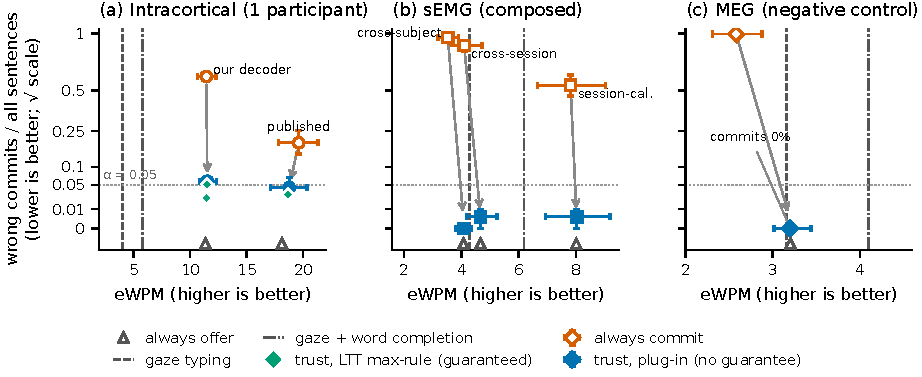
\includegraphics[width=\linewidth]{fig1_teaser.pdf}
  \caption{\textbf{The same trust layer removes almost all wrong commits on three device types.} Each panel plots the wrong-commit rate (share of sentences committed with an error) against effective words per minute (\ewpm{}) of a simulated user. Open markers: always commit the decoder's top sentence. Filled markers: the trust layer on the same decoder output; arrows connect the two. Dashed line: gaze typing alone (no BCI). Dotted line: target $\alpha = 0.05$. Error bars: 95\% bootstrap CIs over trials (a) and sentences (b, c; cluster bootstrap over the 17 unique sentences in c). (a)~Intracortical speech, Brain-to-Text '25, one participant, 816 test trials; ``our decoder'' is our phoneme-to-word decoder, ``published decoder'' is the published LM-rescored sentence. (b)~Forearm sEMG, 551 composed test sentences from 19 participants, three decoder conditions. (c)~MEG typing, 637 test instances (17 unique sentences) from 19 participants, our asynchronous M1-09 decoder.}
  \label{fig:teaser}
\end{figure}

\section{Related work}
\label{sec:related}

\paragraph{Brain-to-text decoders.} Non-invasive MEG decoding of typed sentences reached a mean CER of 0.29 with a keystroke-locked (synchronous) model \citep{levy2026brain2qwerty}. A second version decodes sentences from the continuous recording without key times (asynchronous) and adds an LLM stage \citep{zhang2026brain2qwertyv2}. Other non-invasive work decodes perceived speech \citep{defossez2023decoding} or words with large pre-trained models \citep{jayalath2025unlocking,jayalath2026megxl}. Intracortical decoders reach high accuracy for attempted handwriting \citep{willett2021handwriting}, speech \citep{willett2023speech,card2024accurate,metzger2022spelling} and typing \citep{jude2026bimanual}; public benchmarks expose their phoneme logits \citep{willett2024lessons,card2025data}. Surface EMG typing datasets now exist at scale for the wrist \citep{sivakumar2024emg2qwerty} and the forearm \citep{achituve2025emg}. All these decoders use CTC or a related sequence loss \citep{graves2006ctc} with beam search and an LM \citep{hannun2014deepspeech}. None of them standardises its output, and none decides when its output is safe to commit.

\paragraph{Calibration, selective prediction and abstention.} Modern neural networks are over-confident; temperature scaling is a simple and strong fix \citep{guo2017calibration}, but calibration degrades under dataset shift \citep{ovadia2019trust}. The maximum softmax probability is a strong baseline for detecting errors \citep{hendrycks2017baseline}, and selective classification trades coverage for risk \citep{geifman2017selective}. In BCI, confidence-aware decoding with abstention was shown for EEG speech commands on one device \citep{kim2025confidence}. \todo{G10: add Huang et al.\ 2025 (calibrated alternatives for brain-to-text fusion) once a source page exists.}

\paragraph{Conformal prediction and risk control.} Conformal methods give distribution-free, finite-sample guarantees \citep{angelopoulos2021gentle}. Conformal risk control (CRC) bounds the expected value of a monotone loss \citep{angelopoulos2024crc}; Learn-then-Test (LTT) bounds the risk with high probability by multiple testing \citep{angelopoulos2021ltt}. Under distribution shift, weighted and non-exchangeable variants give approximate bounds \citep{tibshirani2019covariate,barber2023beyond,farinhas2024nonexch}, and online methods adapt a threshold from feedback with long-run guarantees for arbitrary sequences \citep{gibbs2021aci,gibbs2022online,angelopoulos2023pid,feldman2023rolling}. Conformal methods were applied to speech recognition \citep{ernez2023conformal} and to LM outputs and abstention \citep{quach2024conformal,mohri2024factuality,abbasiyadkori2024abstention}. To our knowledge, they have not been applied to the commit decision of neural text entry, nor across device types.

\paragraph{Hallucination in LM-assisted decoding.} LM stages can produce fluent text that the input does not support. In speech recognition this causes real harm \citep{koenecke2024careless}, and generative error correction can replace correct words \citep{chen2023hyporadise}. Reliability-oriented metrics that reward abstention on uncertain input are emerging for ASR \citep{huang2026ras}.

\paragraph{Text-entry and BCI metrics.} BCI work often reports information transfer rate \citep{wolpaw2002bci} or CER/WER; text-entry research uses error metrics such as MSD and KSPC \citep{soukoreff2003metrics}. Studies with gaze-typing users quantify the time cost of selections and corrections \citep{cai2024gaze}. We combine these into an effective-words-per-minute measure with an explicit no-BCI baseline.

\paragraph{Interoperability standards and benchmarks.} Apple's BCI HID profile \citep{applebcihid}, W3C EMMA \citep{w3cemma2009}, Lab Streaming Layer \citep{kothe2024lsl}, BIDS, and IEEE P2731 terminology \citep{ieeep2731} each cover part of the stack: OS input events, multimodal annotation, raw-signal transport, data at rest and vocabulary. Benchmarks such as MOABB and NeuralBench unify decoder evaluation \citep{jayaram2018moabb,banville2026neuralbench}. None of them defines a per-frame decoded-output format with confidence semantics, which is the gap \nts{} fills. \todo{add a BIDS citation (Gorgolewski et al.\ 2016) after it is read.}

\section{Problem setting}
\label{sec:setting}

\paragraph{Items, streams and actions.} An \emph{item} is one attempt to enter one sentence: a \emph{trial} of the intracortical data, an \emph{instance} (one participant typing one sentence) of the MEG data, or a composed \emph{sentence} of the sEMG data. For item $i$, the decoder emits a stream of $F_i$ frames of log-probabilities $\log p_t(v)$ over $V$ tokens. An LM search returns $K = 10$ ranked candidate sentences with scores (the published-sentence gate of \cref{sec:trust} ranks 11: the published sentence and our 10), from which we compute $\hat p_{\mathrm{top1}}$, the calibrated probability of the top candidate. The system then takes one action: \act{commit} the top candidate (sent without further input); \act{offer} up to $k$ candidates for the user to pick; or \act{abstain}, after which the user types with a fallback keyboard (an \act{offer\_words} action, which marks uncertain words, appears only in the ablation). Let $c_i \in \{0,1\}$ indicate that the top candidate differs from the intended sentence (exact match after normalising case and punctuation); for committed items, the simulated user's wrong commit equals $c_i$.

\paragraph{The two error quantities.} Over the $n_{\mathrm{test}}$ test items,
\begin{align}
  \text{wrong-commit rate} &= \#\{\text{wrong commits}\} / n_{\mathrm{test}} \approx \Pr(\text{commit} \wedge \text{wrong}), \\
  \text{error among commits (EAC)} &= \#\{\text{wrong commits}\} / \#\{\text{commits}\} \approx \Pr(\text{wrong} \mid \text{commit}).
\end{align}
The first is the \emph{marginal} risk: how often wrong sentences reach the recipient per sentence attempted. It is monotone in the commit threshold, so CRC and LTT can bound it (\cref{sec:crc}). Committing rarely makes it small, so we always report it with the \emph{commit rate}. The second is the \emph{selective} risk that a user sees in committed text. We report it next to every result and test controllers that bound it (\cref{sec:selective}). \Cref{tab:notation} (\cref{app:notation}) collects the symbols; $\alpha = 0.05$ is the target wrong-commit rate, $\beta$ the target error among commits and $\delta = 0.1$ the failure probability of the high-probability guarantees.

\section{The NeuralTextStream format}
\label{sec:format}

\nts{} (NTS) is the contract between a decoder and any consumer of its output (\cref{fig:arch}). A consumer does not need to know how the decoder works. The full specification, v0.1, is in the repository (\texttt{spec/neuraltextstream-v0.1.md}); here we summarise its design.

\paragraph{Frame core.} A stream of $T$ frames over a vocabulary of $V$ tokens holds a $T \times V$ array \code{log\_probs} of natural-log probabilities (row $t$ is a distribution at frame $t$), the frame times in seconds, the ordered vocabulary \code{vocab}, its type \code{vocab\_type} (\code{char}, \code{key}, \code{word}, \code{phoneme}, \code{command} or \code{other}) and \code{blank\_id}, the index of the CTC blank or \code{null} for non-CTC decoders. Optional fields give the nominal \code{frame\_period}, the algorithmic \code{latency} (look-ahead in seconds; 0 means causal), the producer name and a \code{meta} object. A stream may have $T = 0$.

\paragraph{Semantic conventions.} Following the OpenTelemetry approach of named attribute namespaces, \code{meta} keys use defined prefixes: \code{device.*} (for example \code{device.modality}), \code{decoder.*} (name, version, \code{decoder.causal}, \code{decoder.weights\_sha256}), \code{lm.*}, \code{adapter.*}, \code{calibration.*}, \code{data.derived} and \code{language}. Each field has a stability level; v0.1 is a Development release.

\paragraph{Honest probabilities.} A producer must emit the decoder's own output and must not sharpen or smooth the probabilities for display; calibration is the consumer's job. A number is a probability only if the stream says so. Ground-truth text must not appear in the header or \code{meta} (a leakage rule), and raw signals and direct identifiers stay out of the stream (privacy rules).

\paragraph{Serialisations and conformance.} The reference serialisations are an NPZ file and a JSON Lines streaming form; WebSocket, LSL and HID bridges are sketched. A conformance suite (our code) runs 60 checks, each tied to a specification clause, and reports one of three cumulative levels: \emph{core} (a consumer must accept the stream), \emph{trust-ready} (a trust layer can use it safely: modality, causality, calibration state and language are declared) and \emph{provenance} (a decision can be traced to the producing model: stream id, decoder name, version and weights hash). It ships 52 golden test vectors (32 NPZ, 20 JSON Lines); the reference consumer passes 52 of 52. On synthetic inputs, our MEG and sEMG adapters reach the provenance level and the intracortical adapter reaches trust-ready, because the published online decoder has no weights file to hash. Writing the suite found five bugs in our own producers and ten ambiguities in the specification text, now listed as open questions.

\paragraph{Three device types, no breaking change.} \Cref{tab:devices} lists the three adapters. The MEG decoder emits character CTC frames; the intracortical stream carries the published online phoneme CTC logits (41 tokens, 0.08\,s frames); the sEMG stream has one frame per key press over W3C key codes with \code{blank\_id = null}. Mapping the second and third device types into NTS needed no change to the frame core. The trust harness needed one optional field (the truth in the stream's token space, because phoneme truth differs from the word truth that the user sees), and provenance added optional, non-breaking \code{meta} keys.

\begin{table}[t]
  \centering
  \caption{\textbf{Devices, data and streams.} One adapter per device type maps decoder output into \nts{}. All datasets are public. Test units are those of the trust evaluation.}
  \label{tab:devices}
  \small
  \begin{adjustbox}{max width=\linewidth}\begin{tabular}{@{}llll@{}}
    \toprule
    & \textbf{MEG (typing)} & \textbf{Intracortical (speech)} & \textbf{Forearm sEMG (keys)} \\
    \midrule
    Dataset (licence) & SpanishBCBL (CC BY-NC 4.0) & B2T '25 copy task (CC0) & Toronto sEMG (CC BY 4.0) \\
    Participants & 19 & 1 (T15) & 19 \\
    Test unit & 637 instances, & 816 trials, 14 days & 551 composed \\
     & 17 unique sentences & & sentences \\
    Decoder & own async ConvCTC & published online RNN; & own CNN \\
     & (medium) & own phoneme-to-word route & \\
    NTS \code{vocab\_type} & \code{char} (CTC) & \code{phoneme} (CTC, 41 tokens) & \code{key} (W3C codes) \\
    Frame & one per MEG frame & 0.08\,s & one per key press \\
    \bottomrule
  \end{tabular}\end{adjustbox}
\end{table}

\begin{figure}[t]
  \centering
  \resizebox{\linewidth}{!}{% System architecture of Fidetype (paper version of wiki/diagrams/06 and 07).
% Included from latex/sections/format.tex with \input.
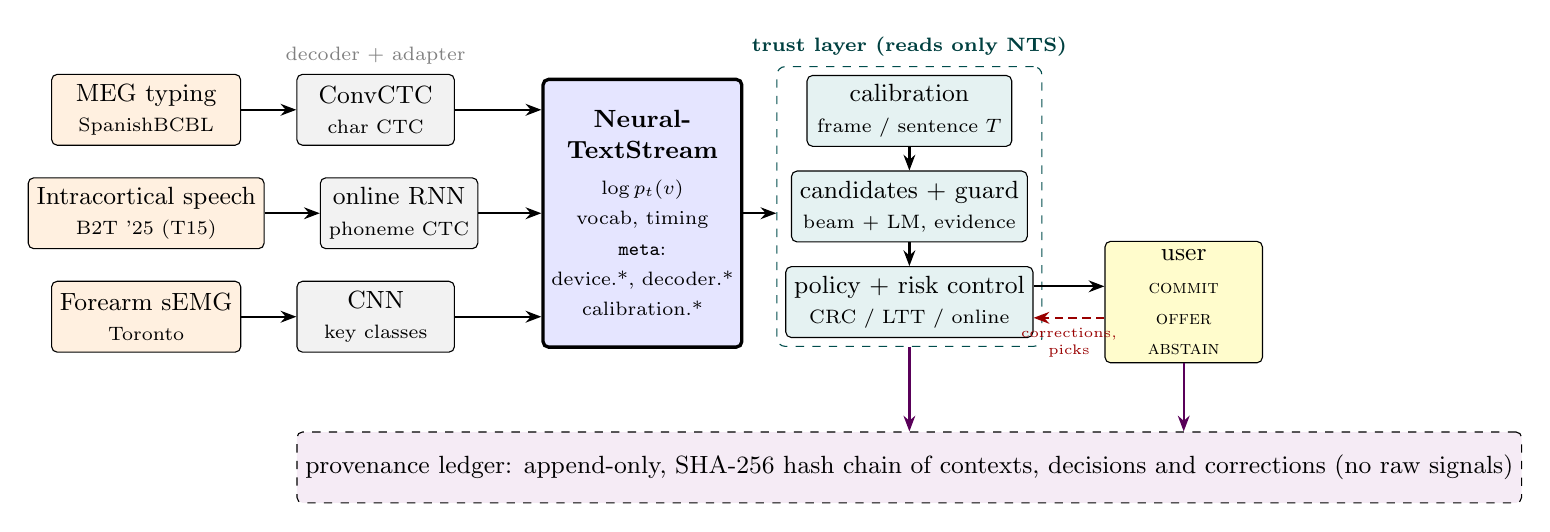
\begin{tikzpicture}[
  font=\small,
  box/.style={draw, rounded corners=2pt, align=center, minimum height=9mm, inner sep=3pt, fill=white},
  dev/.style={box, fill=orange!12, minimum width=24mm},
  ada/.style={box, fill=gray!10, minimum width=20mm},
  nts/.style={box, fill=blue!10, minimum width=22mm, minimum height=34mm, very thick},
  tl/.style={box, fill=teal!10, minimum width=26mm},
  usr/.style={box, fill=yellow!20, minimum width=20mm},
  led/.style={box, fill=violet!8, minimum width=118mm, dashed},
  arr/.style={-{Stealth[length=2mm]}, thick},
  fb/.style={-{Stealth[length=2mm]}, thick, densely dashed, red!60!black},
  node distance=4mm and 7mm]
  % devices
  \node[dev] (meg) {MEG typing\\\scriptsize SpanishBCBL};
  \node[dev, below=of meg] (ic) {Intracortical speech\\\scriptsize B2T '25 (T15)};
  \node[dev, below=of ic] (emg) {Forearm sEMG\\\scriptsize Toronto};
  % decoders + adapters
  \node[ada, right=of meg] (dmeg) {ConvCTC\\\scriptsize char CTC};
  \node[ada, right=of ic] (dic) {online RNN\\\scriptsize phoneme CTC};
  \node[ada, right=of emg] (demg) {CNN\\\scriptsize key classes};
  % NTS
  \node[nts, right=8mm of dic] (nts) {\textbf{Neural-}\\\textbf{TextStream}\\[2pt]\scriptsize $\log p_t(v)$\\\scriptsize vocab, timing\\\scriptsize \texttt{meta}:\\\scriptsize device.*, decoder.*\\\scriptsize calibration.*};
  % trust layer
  \node[tl, right=8mm of nts, yshift=13mm] (cal) {calibration\\\scriptsize frame / sentence $T$};
  \node[tl, below=3mm of cal] (cand) {candidates + guard\\\scriptsize beam + LM, evidence};
  \node[tl, below=3mm of cand] (pol) {policy + risk control\\\scriptsize CRC / LTT / online};
  \node[draw, rounded corners=3pt, dashed, teal!60!black, fit=(cal)(cand)(pol), inner sep=3pt, label={[teal!50!black,font=\scriptsize\bfseries]above:trust layer (reads only NTS)}] (tlbox) {};
  % user
  \node[usr, right=9mm of pol] (user) {user\\[1pt]\scriptsize \textsc{commit}\\\scriptsize \textsc{offer}\\\scriptsize \textsc{abstain}};
  % ledger
  \node[led, below=10mm of demg.south west, anchor=north west] (led) {provenance ledger: append-only, SHA-256 hash chain of contexts, decisions and corrections (no raw signals)};
  % arrows
  \foreach \a/\b in {meg/dmeg, ic/dic, emg/demg} \draw[arr] (\a) -- (\b);
  \foreach \a in {dmeg, dic, demg} \draw[arr] (\a.east) -- (\a.east -| nts.west);
  \node[font=\scriptsize, gray, above=0mm of dmeg] {decoder + adapter};
  \draw[arr] (nts.east) -- (nts.east -| tlbox.west);
  \draw[arr] (cal) -- (cand);
  \draw[arr] (cand) -- (pol);
  \draw[arr] ([yshift=2mm]pol.east) -- ([yshift=2mm]pol.east -| user.west);
  \draw[fb] ([yshift=-2mm]user.west) -- node[below, font=\tiny, align=center] {corrections,\\picks} ([yshift=-2mm]user.west -| pol.east);
  \draw[arr, violet!70!black] (tlbox.south) -- (tlbox.south |- led.north);
  \draw[arr, violet!70!black] (user.south) -- (user.south |- led.north);
\end{tikzpicture}
}
  \caption{\textbf{Architecture.} Each device's decoder emits a \nts{} through a small adapter. The trust layer reads only the stream: it calibrates confidence, builds candidate sentences with a neural-evidence guard, and chooses an action under a risk-control rule. The user's corrections and picks (dashed) feed the online re-calibration. Every context, decision and correction goes to an append-only, hash-chained provenance ledger that stores no raw signals.}
  \label{fig:arch}
\end{figure}

\section{The trust layer}
\label{sec:trust}

The trust layer reads one \nts{} per sentence attempt and returns one action. It never reads raw signals or decoder internals. \Cref{fig:decision} shows the decision flow.

\subsection{Calibration}
Decoder log-probabilities are often over-confident. We fit a frame temperature $T_f$ that rescales every frame, $\tilde p_t(v) \propto p_t(v)^{1/T_f}$, by minimising the negative log-likelihood of the truth on fit data, and a sentence temperature $T_s$ for the sentence-level confidence $\hat p_{\mathrm{top1}}$, the normalised probability of the top candidate among the n-best \citep{guo2017calibration}. We report the expected calibration error (ECE) of $\hat p_{\mathrm{top1}}$ before and after.

\subsection{Candidates and neural-evidence guard}
Candidate sentences come from a CTC prefix beam search with a character 6-gram LM and a word unigram, both trained on Tatoeba sentences, and an n-best list (n = 10) \citep{graves2006ctc,hannun2014deepspeech}. For the published intracortical sentences, the candidate is the given text. Because the LM can write fluent text from any input, a guard scores how much of each candidate the LM invented. It combines two signals: the share of the candidate's characters whose posterior under the calibrated frames alone (no LM) is low (\emph{low evidence}), and one minus the posterior-weighted word agreement between the top candidate and the other n-best candidates (\emph{n-best inconsistency}); the guard risk is the maximum of the two weighted signals. A candidate with high guard risk cannot be committed.

\subsection{Decision policy}
The policy chooses one of four actions: \act{commit} the top candidate; \act{offer} the top $k$ candidates for the user to pick; \act{offer\_words}, an offer with uncertain words highlighted; or \act{abstain}, after which the user types the sentence with the fallback keyboard. The thresholds (commit probability, guard risk, offer size, abstain risk, fallback) are chosen on fit data from a small grid to maximise \ewpm{} (\cref{sec:protocol}) subject to a wrong-commit rate $\le 0.05$ on the fit data. This plug-in fit has no guarantee on new data, which motivates \cref{sec:crc}.

\subsection{Finite-sample risk control for the commit threshold}
\label{sec:crc}
Let $s_i$ be the score of item $i$ ($\hat p_{\mathrm{top1}}$ if the other policy rules allow a commit, else $-\infty$) and $\lambda$ the commit threshold. The loss is $L_i(\lambda) = c_i$ if $s_i \ge \lambda$ (with $c_i = 1$ if the top candidate is wrong) and $f_i$ otherwise (the loss of the non-commit action, 0 here), made monotone in $\lambda$ by taking $\max(c_i, f_i)$. On $n$ calibration items with known truth, conformal risk control \citep{angelopoulos2024crc} chooses
\begin{equation}
  \hat\lambda_{\mathrm{CRC}} = \inf\Bigl\{\lambda : \tfrac{n}{n+1}\hat R_n(\lambda) + \tfrac{1}{n+1} \le \alpha\Bigr\},
\end{equation}
where $\hat R_n$ is the empirical risk. If calibration and test items are exchangeable, $\mathbb{E}[L_{n+1}(\hat\lambda_{\mathrm{CRC}})] \le \alpha$. No feasible $\lambda$ exists for $n < 1/\alpha - 1$ (19 for $\alpha = 0.05$); the layer then never commits. Learn-then-Test \citep{angelopoulos2021ltt} instead tests $H_0\colon R(\lambda) > \alpha$ along a decreasing grid with exact binomial p-values and fixed-sequence testing, which gives $\Pr(R(\hat\lambda_{\mathrm{LTT}}) \le \alpha) \ge 1 - \delta$. Any threshold above $\hat\lambda$ keeps the guarantee, so the layer can combine CRC with the \ewpm{}-tuned threshold as $\hat\lambda = \max(\lambda_{\mathrm{tuned}}, \hat\lambda_{\mathrm{CRC}})$. The other parts of the pipeline (temperatures, guard, other thresholds) are fitted on separate data. We use $\alpha = 0.05$ and $\delta = 0.1$ throughout.

\subsection{Online re-calibration under drift}
\label{sec:online}
Exchangeability fails when a session drifts. The online controller re-fits the threshold during the session from user feedback (\cref{fig:online}). Which feedback exists depends on the action: a corrected commit reveals a wrong commit; an uncorrected commit is right only if silence means right; an offer reveals the truth when the user picks or retypes; an abstention reveals nothing unless the final text is logged. The controller therefore accepts two feedback levels: the \emph{realised loss} of committed items, and, when the final text is known, the counterfactual commit loss of non-committed items. Feedback can arrive late and out of order. \Cref{tab:online} lists the four methods.

\begin{table}[t]
  \centering
  \caption{\textbf{Online re-calibration methods for the commit threshold.} $L_t$: realised loss at item $t$; $T$: number of items in the session. The two \texttt{aci} variants bound the long-run average loss for any sequence of items, without exchangeability.}
  \label{tab:online}
  \small
  \begin{adjustbox}{max width=\linewidth}\begin{tabular}{@{}llll@{}}
    \toprule
    \textbf{Method} & \textbf{Update} & \textbf{Guarantee} & \textbf{Feedback} \\
    \midrule
    \texttt{window} & CRC on the last $N$ items with known truth & approximate & full \\
    \texttt{decay} & weighted CRC, weights $\rho^{\text{age}}$ \citep{barber2023beyond,farinhas2024nonexch} & approximate & full \\
    \texttt{aci} & $\lambda_{t+1} = \max(\lambda_{\min}, \lambda_t + \eta(L_t - \alpha))$ & $\frac1T\sum L_t \le \alpha + \frac{\lambda_{T+1} - \lambda_1}{\eta T}$ & realised only \\
    \texttt{aci\_window} & window CRC at level $\alpha_t$; $\alpha_{t+1} = \alpha_t + \gamma(\alpha - L_t)$ & $\frac1T\sum L_t \le \alpha + \frac{\alpha_1 - \alpha_{T+1}}{\gamma T}$ & full + realised \\
    \bottomrule
  \end{tabular}\end{adjustbox}
\end{table}

The \texttt{aci} rule follows adaptive conformal inference and online risk control \citep{gibbs2021aci,angelopoulos2023pid,feldman2023rolling}; \texttt{aci\_window} applies the ACI update to the level of a windowed CRC \citep{gibbs2021aci}. We use $N = 200$, $\rho = 0.99$, $\eta = 0.05$ and $\gamma = 0.005$, fixed before the evaluation. These bounds are long-run averages over the $T$ items of a session; they say nothing about short windows, and they cover only the errors that the system observes. A wrong commit that the user does not notice (a \emph{silent error}) is outside them.

\subsection{Provenance ledger}
\label{sec:ledger}
Each decision is appended to a JSON Lines ledger. Entry 0 is a genesis record; \emph{context} entries are content-addressed (their id is the SHA-256 of the context) and hold the adapter, decoder (name, version, weights hash, training data and licence), LM, calibration (temperatures, risk-control method, $\alpha$, $\delta$, threshold, $n$) and policy versions; \emph{decision} entries hold the action, scores, a hash of the \nts{} and its frame range; \emph{correction} entries link to the decision they correct and store the edit distance. Each entry stores \code{prev\_hash} and its own SHA-256 over the canonical JSON, so any edit, deletion or reordering breaks the chain; a separately stored head anchor detects truncation. The ledger stores no raw signals (numeric arrays longer than 64 values are rejected), stores text as a keyed hash by default, and pseudonymises subject and session ids. It is tamper-evident, not tamper-proof: there is no signature in v0.

\begin{figure}[t]
  \centering
  \resizebox{\linewidth}{!}{% Trust decision flow for one sentence: COMMIT / OFFER / ABSTAIN with the CRC threshold.
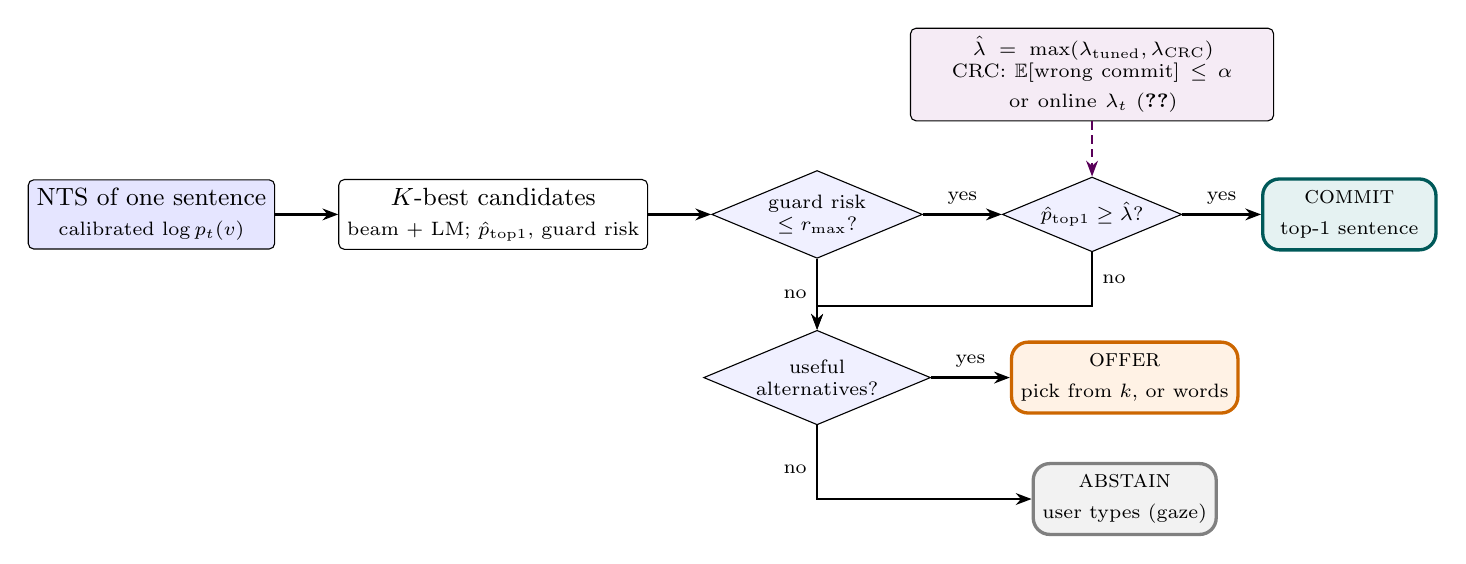
\begin{tikzpicture}[
  font=\small,
  box/.style={draw, rounded corners=2pt, align=center, fill=white, minimum height=8mm, inner sep=3pt},
  dec/.style={draw, diamond, aspect=2.4, align=center, fill=blue!6, inner sep=1pt, font=\scriptsize},
  act/.style={draw, rounded corners=6pt, align=center, minimum width=22mm, minimum height=9mm, very thick},
  arr/.style={-{Stealth[length=2mm]}, thick},
  node distance=5mm and 8mm]
  \node[box, fill=blue!10] (in) {NTS of one sentence\\\scriptsize calibrated $\log p_t(v)$};
  \node[box, right=of in] (cand) {$K$-best candidates\\\scriptsize beam + LM; $\hat p_{\mathrm{top1}}$, guard risk};
  \node[dec, right=of cand] (g) {guard risk\\$\le r_{\max}$?};
  \node[dec, right=10mm of g] (lam) {$\hat p_{\mathrm{top1}} \ge \hat\lambda$?};
  \node[act, draw=teal!70!black, fill=teal!10, right=10mm of lam] (commit) {\textsc{commit}\\\scriptsize top-1 sentence};
  \node[dec, below=9mm of g] (off) {useful\\alternatives?};
  \node[act, draw=orange!80!black, fill=orange!10, right=10mm of off] (offer) {\textsc{offer}\\\scriptsize pick from $k$, or words};
  \node[act, draw=gray, fill=gray!10, below=6mm of offer] (abst) {\textsc{abstain}\\\scriptsize user types (gaze)};
  \node[box, fill=violet!8, above=7mm of lam, text width=44mm] (thr) {\scriptsize $\hat\lambda = \max(\lambda_{\mathrm{tuned}}, \lambda_{\mathrm{CRC}})$\\\scriptsize CRC: $\mathbb{E}[\text{wrong commit}] \le \alpha$\\\scriptsize or online $\lambda_t$ (\cref{sec:online})};
  \draw[arr] (in) -- (cand);
  \draw[arr] (cand) -- (g);
  \draw[arr] (g) -- node[above, font=\scriptsize] {yes} (lam);
  \draw[arr] (lam) -- node[above, font=\scriptsize] {yes} (commit);
  \draw[arr] (g) -- node[left, font=\scriptsize] {no} (off);
  \draw[arr] (lam) |- node[pos=0.25, right, font=\scriptsize] {no} ($(off.north)+(0,3mm)$) -- (off.north);
  \draw[arr] (off) -- node[above, font=\scriptsize] {yes} (offer);
  \draw[arr] (off) |- node[pos=0.3, left, font=\scriptsize] {no} (abst);
  \draw[arr, violet!70!black, densely dashed] (thr.south) -- (lam.north);
\end{tikzpicture}
}
  \caption{\textbf{Trust decision for one sentence.} Candidates come from the calibrated stream. A candidate is committed only if the neural-evidence guard accepts it and its calibrated confidence reaches the threshold $\hat\lambda$, which is the larger of the \ewpm{}-tuned threshold and the CRC threshold (or the online threshold $\lambda_t$). Otherwise the layer offers alternatives or abstains, and the user types with the fallback keyboard.}
  \label{fig:decision}
\end{figure}

\begin{figure}[t]
  \centering
  \resizebox{0.95\linewidth}{!}{% Online re-calibration loop of the COMMIT threshold (aci and aci_window).
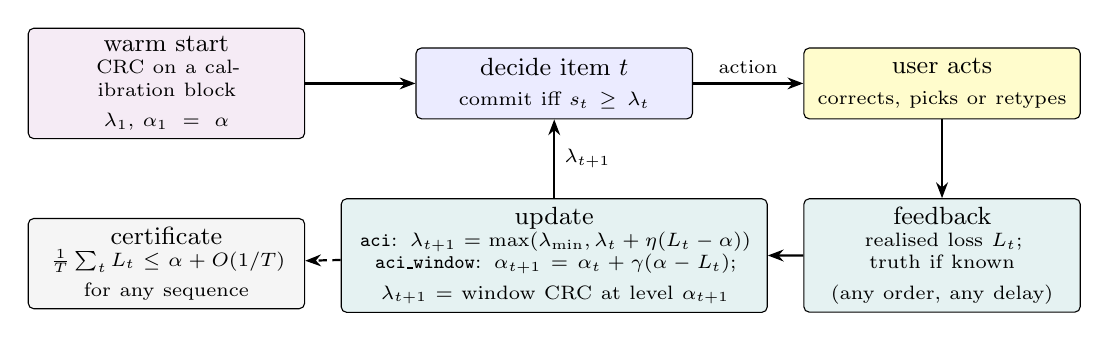
\begin{tikzpicture}[
  font=\small,
  box/.style={draw, rounded corners=2pt, align=center, fill=white, minimum height=9mm, inner sep=3pt, text width=33mm},
  arr/.style={-{Stealth[length=2mm]}, thick},
  node distance=6mm and 14mm]
  \node[box, fill=violet!8] (warm) {warm start\\\scriptsize CRC on a calibration block\\\scriptsize $\lambda_1$, $\alpha_1 = \alpha$};
  \node[box, fill=blue!8, right=of warm] (dec) {decide item $t$\\\scriptsize commit iff $s_t \ge \lambda_t$};
  \node[box, fill=yellow!20, right=of dec] (user) {user acts\\\scriptsize corrects, picks or retypes};
  \node[box, fill=teal!10, below=10mm of user] (fb) {feedback\\\scriptsize realised loss $L_t$; truth if known\\\scriptsize (any order, any delay)};
  \node[box, fill=teal!10, below=10mm of dec, text width=52mm] (upd) {update\\\scriptsize \texttt{aci}: $\lambda_{t+1} = \max(\lambda_{\min}, \lambda_t + \eta (L_t - \alpha))$\\\scriptsize \texttt{aci\_window}: $\alpha_{t+1} = \alpha_t + \gamma(\alpha - L_t)$;\\\scriptsize $\lambda_{t+1}$ = window CRC at level $\alpha_{t+1}$};
  \node[box, fill=gray!8, below=10mm of warm] (cert) {certificate\\\scriptsize $\frac{1}{T}\sum_t L_t \le \alpha + O(1/T)$\\\scriptsize for any sequence};
  \draw[arr] (warm) -- (dec);
  \draw[arr] (dec) -- node[above, font=\scriptsize] {action} (user);
  \draw[arr] (user) -- (fb);
  \draw[arr] (fb) -- (upd);
  \draw[arr] (upd) -- node[right, font=\scriptsize] {$\lambda_{t+1}$} (dec);
  \draw[arr, densely dashed] (upd) -- (cert);
\end{tikzpicture}
}
  \caption{\textbf{Online re-calibration loop.} A short calibration block gives the starting threshold. After each item, the realised loss (and the truth, if the final text is known) updates the threshold. For \texttt{aci} and \texttt{aci\_window}, the running wrong-commit rate is bounded by $\alpha$ plus a term that shrinks as $1/T$, for any sequence of items.}
  \label{fig:online}
\end{figure}

\section{Evaluation protocol}
\label{sec:protocol}

\subsection{Effective words per minute}
Error rates compare decoders but do not tell whether a user saves time. We therefore simulate a user who reads the system output, accepts or corrects a commit, picks from an offer, or types the sentence with a fallback keyboard. For item $i$ with intended sentence $y_i$, the simulation returns the total time $t_i$ (input, reading, selections, corrections and retyping) and the final text. The effective words per minute are
\begin{equation}
  \text{\ewpm{}} = 60 \cdot \frac{\sum_i \mathbf{1}[\text{final text}_i = y_i]\;\mathrm{words}(y_i)}{\sum_i t_i},
\end{equation}
a ratio of sums over all test items in which a sentence counts only if it is exactly right at the end. Like the BCI utility metric \citep{dalseno2010utility}, \ewpm{} charges the time needed to fix errors. A \emph{silent error} is a wrong final text that the user did not correct; it reaches the recipient and counts zero words. \ewpm{} does not price the harm of a silent error beyond the lost words, so we report the silent-error rate separately.

\subsection{User model and baselines}
The user model is a gaze-typing user. The fallback keyboard runs at 20 characters per minute, and scanning and selecting one of $k = 3$ word alternatives takes 4.5\,s; both are matched to measurements of one eye-gaze typing user with ALS \citep{cai2024gaze}. All other time costs are assumptions (\cref{tab:user}). The neural input runs at a device-specific speed: the measured 159.3 characters per minute of the intracortical participant; 75.8 characters per minute for sEMG (the 0.792\,s median press period); and 152 characters per minute for MEG (the healthy participants' typing speed).

\paragraph{Silent errors and the asymmetry between commit and offer.} After a \act{commit}, the user reads the sentence and misses each wrong word independently with probability 0.05; a missed wrong word becomes a silent error. After an \act{offer}, the user compares the candidates on purpose and sees every error, and chooses the cheapest of picking, fixing words or retyping, using the true costs. This asymmetry favours offers. It encodes the hypothesis that committed text is checked less carefully than offered text, which is not measured. The model does not make fluent wrong sentences harder to notice than garbled ones: a sentence with more wrong words is more likely to keep at least one of them. \Cref{sec:res-main} reports how the MEG conclusions change under other user-model settings. \todo{R1: user-model sensitivity grid on all three devices, a symmetric-offer variant and a misspecified-user evaluation without refitting.}

\paragraph{Population mismatch.} The fallback and selection costs are those of an eye-gaze user with ALS. This matches the intracortical participant, who has ALS. The MEG and sEMG decoders, however, read overt typing by able-bodied people, who would not need a gaze keyboard. For these two devices, \ewpm{} answers a hypothetical question: how fast would a gaze-typing user be with a decoder that has this error profile at this input rate?

\paragraph{Baselines.} \emph{Gaze typing only}: the same user types every sentence with the fallback keyboard and no BCI. This baseline is error-free and has no reading or correction time, which slightly favours it, but it also has no LM-based word prediction, which favours the BCI arms; LM prediction is known to speed up gaze typing \citep{ward2000dasher,cai2024gaze}. \todo{R1: LM-assisted gaze baseline (same 6-gram, word completion with $k = 3$ slots).} \emph{Always commit}: commit the top candidate of every item. \emph{Always offer}: offer the top candidates of every item and never commit; this is what most BCI spellers and AAC systems do.

\subsection{Datasets and splits}
\paragraph{Intracortical speech (Brain-to-Text '25).} The public copy-task file holds the online phoneme CTC logits, the cue sentences and the published LM-rescored sentences of participant T15, an implant recipient in the BrainGate2 clinical trial, for 1,718 trials over 15 days \citep{card2024accurate,card2025data}. We use the 1,628 trials with the 125,000-word vocabulary, which span 14 days; the 90 trials with a 50-word vocabulary are excluded. The file has no trial time stamps; we take the file order within each day as the trial order. We fit on the first half of each day (812 trials) and test on the second half (816 trials); one sentence occurs in both halves. Inside the fit half, the frame and sentence temperatures use the first half of the fit trials and the policy uses all of them. We evaluate two decoders: our own phoneme-to-word decoder (phoneme beam, CMUdict lexicon, Tatoeba word unigram and character LM; test WER 0.149) and the published sentence (test WER 0.043), which we gate as described in \cref{sec:trust}.

\paragraph{Forearm sEMG (Toronto).} The dataset holds isolated key presses from 19 participants over two days \citep{achituve2025emg,achituve2024data}. Because it has no continuous typing, we compose sentences from single presses, with oracle press timing and no inter-key context: one real press window per character, at the median press period. Sentences are held-out Tatoeba sentences that the LM did not see; exact overlap is excluded, but near-duplicates were not checked, and the style matches the LM corpus. Each participant contributes 30 fit sentences built from presses of the first day-2 recording of each letter, and up to 30 test sentences from later recordings (570 fit, 551 test). With about 10 presses per letter per pool, a press can appear in several test sentences, so sentence-level intervals are too narrow and participant intervals are primary. A CNN classifies each press. Three conditions vary how much of the user's data the decoder saw: \emph{session-calibrated} (day 1 plus half of the day-2 recordings, cross-fitted: the decoder that predicts the test presses is trained on the first recordings, and the fit sentences are predicted by the decoder trained on the later ones), \emph{cross-session} (day 1 only) and \emph{cross-subject} (4-fold leave-participants-out). Within the fit sentences, one half (A) fits the temperatures and the LM weight and the other half (B) fits the policy; CRC and LTT use the last 142 sentences of half B and the grid the first half.

\paragraph{MEG typing (SpanishBCBL).} Healthy participants typed memorised Spanish sentences in an MEG scanner \citep{levy2026brain2qwerty,spanishbcbl}. We use 19 participants and split by a hash of the sentence text into 101 training, 11 validation and 17 test sentences. The split is within participants: the same 19 people appear in training and test, with different sentences. No test sentence appears in training or in the LM text. The test set has 637 instances of the 17 sentences; all trust parameters are fitted on the 437 validation instances of 11 sentences. Our asynchronous ConvCTC decoder (convolutional front end and 4 Conformer layers of width 256 \citep{gulati2020conformer}) receives the MEG segment from 0.4\,s before the first key press to 0.5\,s after the last, its length and the participant index, but no key times at inference. It uses key times as auxiliary training labels, and the sentence bounds come from the keyboard log, so it is not a free-running decoder and cannot be trained for a user who cannot type (\cref{app:meg}). The trust harness decodes its streams with a fixed beam setting (LM weight 0.5, frame temperature fitted on validation) whose top-1 CER is 0.522, higher than the 0.475 of the beam setting tuned on validation CER (\cref{tab:decoders}). A synchronous decoder with oracle key times gives the same trust results (\cref{app:meg}).

\subsection{Controls}
\emph{Decoder controls} show that the decoders use the neural signal: shuffled MEG, zero input, and a decoder trained with permuted labels. \emph{Trust-layer controls} come in two classes. \emph{Signal-destroying controls} keep the stream format but remove the neural information: frame-shuffled streams, near-uniform streams, zero-input decoder output and a permuted-label decoder. A stream-only layer should not commit these. The \emph{intent-mismatch control} is the real stream of a different sentence by the same participant. It carries genuine neural evidence, only for a sentence the user did not intend now, so a stream-only layer cannot detect it.

\subsection{Statistics}
We report 95\% percentile bootstrap confidence intervals and paired differences on the same items. The resampling unit is stated with every interval: trials \texttt{[trial]} and days \texttt{\{day\}} for Brain-to-Text '25; sentences \texttt{[sent]} and participants \texttt{\{participant\}} for sEMG, where participants are primary; for MEG trust results, unique sentences (cluster bootstrap over the 17 test sentences), participants, and both at once (two-way), with the two-way interval primary for comparisons with gaze typing. MEG decoder CER intervals over instances are too narrow and are not used for inference. We name two primary endpoints per device: the wrong-commit rate of the trust layer and the paired \ewpm{} difference between the trust layer and gaze typing. All other intervals are descriptive and not corrected for multiplicity. Decoder settings, user-model values, the policy grid, $\alpha$, $\delta$ and the online step sizes were fixed in the experiment configurations before the evaluation runs. The ``noticed errors only'' online runs were added after the first run without changing any setting. Every decoder and trust run uses one seed and one fit/test split. \todo{R1: decoder seeds and repeated fit/test splits; sentence-cluster CIs for MEG CER.}

\section{Results}
\label{sec:results}

\subsection{The decoders use the neural signal}
\label{sec:res-decoders}

Before we evaluate the trust layer, we check that each decoder reads its input (\cref{tab:decoders}). Our asynchronous MEG decoder reached a test CER of 0.506 with greedy decoding (0.495 $\pm$ 0.020 SEM over the 19 participants) and 0.475 with beam search and the character LM (\cref{fig:megcer}). With shuffled MEG the CER rose to 0.760 and with zero input to 0.925; the paired shuffled-minus-real gap was $+0.254$ \ci{+0.241}{+0.265} (instances). On the 11 test sentences with no close training variant, CER was 0.519 (greedy) and 0.492 (beam + LM), so near-variant sentences changed the headline by about 0.013 and 0.017. A longer training schedule did not help (r5 minus r4b, greedy $+0.009$ \ci{+0.003}{+0.015}). For reference, the published asynchronous encoder reports $0.59 \pm 0.02$ on SpanishBCBL \citep{zhang2026brain2qwertyv2}; this is not a head-to-head comparison, because the test splits differ and our decoder uses key times as training labels. On B2T '25, our phoneme-to-word route reached WER 0.149 and the published decoder 0.043. On sEMG, the CNN reached key accuracies of 0.299 (session-calibrated), 0.168 (cross-session) and 0.209 (cross-subject); with permuted training labels it fell to 0.022, the chance level.

\begin{table}[t]
  \centering
  \caption{\textbf{Decoder quality and input controls.} CER/WER on the test sets; lower is better. MEG intervals are over instances. ``Far'' = the 11 MEG test sentences with no close training variant.}
  \label{tab:decoders}
  \small
  \begin{adjustbox}{max width=\linewidth}\begin{tabular}{@{}llll@{}}
    \toprule
    \textbf{Device} & \textbf{Decoder} & \textbf{Real input} & \textbf{Controls} \\
    \midrule
    MEG & M1-09 async, greedy (CER) & 0.506 (participants 0.495 $\pm$ 0.020) & shuffled 0.760, zeros 0.925 \\
    MEG & M1-09 async, beam + LM (CER) & 0.475 (participants 0.462 $\pm$ 0.022) & --- \\
    MEG & far sentences, greedy / beam (CER) & 0.519 / 0.492 & --- \\
    MEG & v2 Encoder Async \citep{zhang2026brain2qwertyv2} (CER) & $0.59 \pm 0.02$ (other split) & --- \\
    B2T '25 & our phoneme-to-word route (WER) & 0.149 & --- \\
    B2T '25 & published decoder (WER) & 0.043 (0.0434 pooled, 1,718 trials) & --- \\
    sEMG & CNN, session-cal.\ / cross-session / cross-subject & key accuracy 0.299 / 0.168 / 0.209 & permuted labels 0.022 \\
    \bottomrule
  \end{tabular}\end{adjustbox}
\end{table}

\begin{figure}[t]
  \centering
  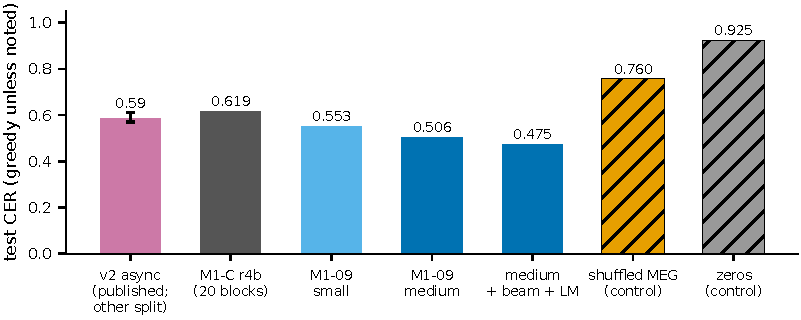
\includegraphics[width=\linewidth]{fig_meg_cer.pdf}
  \caption{\textbf{Our asynchronous MEG decoder uses the signal.} Test CER on SpanishBCBL (637 instances, 17 unique sentences, 19 participants), mean over sentences. The published v2 value (mean $\pm$ SEM over participants) uses a different test split and is shown for orientation only. Hatched bars: input controls for the medium model (greedy). \todo{G2: add seed variability.}}
  \label{fig:megcer}
\end{figure}

\subsection{The trust layer cuts wrong commits on three device types}
\label{sec:res-main}

\Cref{tab:main} and \cref{fig:teaser,fig:ewpm} give the main result.

\paragraph{Intracortical speech.} Always committing the top sentence of our decoder gave 11.45 \ewpm{} and a wrong-commit rate of 0.610. The trust layer, on the same output, gave 11.55 \ewpm{} and a wrong-commit rate of 0.059 \ci{0.043}{0.075}. The paired \ewpm{} difference was \ci{-0.11}{+0.30} and the wrong-commit difference \ci{-0.587}{-0.516} (trials). Used as a gate on the published LM-rescored sentences, the layer reduced the wrong-commit rate from 0.194 to 0.044 \ci{0.031}{0.059} at a speed cost of 4.3\% (paired \ewpm{} \ci{-0.98}{-0.72}). All BCI policies were far faster than gaze typing alone (4.08 \ewpm{}; trust minus gaze \ci{+6.96}{+7.97}, gate minus gaze \ci{+13.81}{+15.53}).

\paragraph{Forearm sEMG.} In all three decoder conditions the trust layer reduced the wrong-commit rate from 0.541, 0.882 and 0.962 to 0.004, 0.004 and 0.000, and it raised \ewpm{} over always-commit (paired differences \ci{+0.05}{+0.38}, \ci{+0.44}{+0.72} and \ci{+0.43}{+0.67}, sentences). The layer committed only 0--4\% of sentences; the speed gain came from offers, from which the user picks a candidate. Only the session-calibrated decoder clearly beat gaze typing (8.02 vs 4.27 \ewpm{}; trust minus gaze \ci{+3.38}{+4.16}). The cross-subject condition stayed below gaze typing (4.08).

\paragraph{MEG.} With our asynchronous decoder, the LM top sentence was right for 2 of 637 test instances (0.0031), and the true sentence was in the 10-best list for 1.6\%. Always committing the top sentence therefore gave a wrong-commit rate of 0.997 and 2.580 \ewpm{} \ci{2.41}{2.76}. The trust layer committed nothing (wrong-commit 0) and offered candidates instead, which gave 3.203 \ewpm{} \ci{3.07}{3.36} (sentences; \{3.08, 3.37\} over participants), $+0.62$ over always-commit \ci{+0.49}{+0.75}. Gaze typing alone gave 3.155 \ci{3.02}{3.29}. The paired difference to gaze typing was $+0.05$, with CIs of \ci{-0.04}{+0.15} over sentences and \ci{-0.07}{+0.22} over participants: this is parity, not a gain. Per participant, the trust layer was above gaze typing for 10 of 19 participants and below for 9 (range $-0.34$ to $+1.16$ \ewpm{}). The synchronous M1-15 decoder with oracle key timing gave the same picture (trust 3.229, always-commit 2.714; trust minus gaze \ci{-0.02}{+0.18} over sentences).

\begin{table}[t]
  \centering
  \caption{\textbf{Safety and speed on three device types (test sets).} \ewpm{} with 95\% bootstrap CIs; square brackets: trials (B2T '25) or sentences (sEMG; MEG, cluster bootstrap over the 17 unique sentences); curly brackets: days (B2T '25) or participants (sEMG, MEG). The MEG wrong-commit CI is over sentences. Wrong-commit: share of items committed with an error. Silent error: wrong commit not noticed by the simulated user. ``---'': not computed.}
  \label{tab:main}
  \small
  \begin{adjustbox}{max width=\linewidth}\begin{tabular}{@{}lllll@{}}
    \toprule
    \textbf{Device / condition} & \textbf{Policy} & \textbf{\ewpm{} [CI] \{CI\}} & \textbf{Wrong-commit} & \textbf{Silent} \\
    \midrule
    B2T '25, our decoder & always commit top-1 & 11.45 \ci{10.95}{12.04} \{10.72, 12.32\} & 0.610 \ci{0.574}{0.645} & 0.044 \\
     & trust & 11.55 \ci{11.03}{12.06} \{10.85, 12.38\} & 0.059 \ci{0.043}{0.075} & 0.002 \\
    B2T '25, published & always commit & 19.61 \ci{18.68}{20.51} \{17.76, 21.45\} & 0.194 \ci{0.167}{0.222} & 0.025 \\
     & trust gate & 18.77 \ci{17.88}{19.62} \{17.05, 20.46\} & 0.044 \ci{0.031}{0.059} & 0.004 \\
    B2T '25 & gaze typing only & 4.08 \ci{4.04}{4.12} & 0 & 0 \\
    \midrule
    sEMG session-cal. & always commit LM top-1 & 7.81 \ci{7.36}{8.30} \{6.60, 9.01\} & 0.541 & 0.060 \\
     & trust & 8.02 \ci{7.63}{8.45} \{6.90, 9.15\} & 0.004 & 0.000 \\
    sEMG cross-session & always commit LM top-1 & 4.10 \ci{3.89}{4.34} \{3.59, 4.70\} & 0.882 & 0.149 \\
     & trust & 4.68 \ci{4.52}{4.86} \{4.21, 5.25\} & 0.004 & 0.000 \\
    sEMG cross-subject & always commit LM top-1 & 3.53 \ci{3.37}{3.72} & 0.962 & 0.167 \\
     & trust & 4.08 \ci{3.98}{4.20} & 0.000 & 0.000 \\
    sEMG & gaze typing only & 4.27 & 0 & 0 \\
    \midrule
    MEG (async M1-09) & always commit LM top-1 & 2.580 \ci{2.41}{2.76} \{2.41, 2.79\} & 0.997 \ci{0.990}{1.000} & 0.235 \\
     & trust & 3.203 \ci{3.07}{3.36} \{3.08, 3.37\} & 0.000 & 0.000 \\
    MEG & gaze typing only & 3.155 \ci{3.02}{3.29} & 0 & 0 \\
    \bottomrule
  \end{tabular}\end{adjustbox}
\end{table}

\begin{figure}[t]
  \centering
  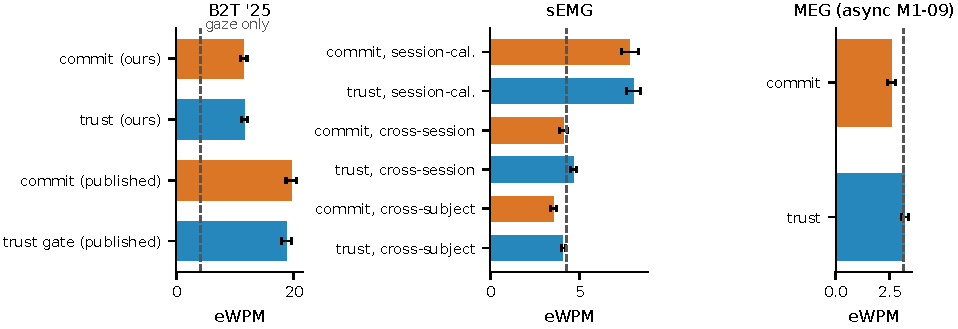
\includegraphics[width=\linewidth]{fig_ewpm_policies.pdf}
  \caption{\textbf{Speed per policy and device.} \ewpm{} of the simulated user; orange: always commit, blue: trust layer. Error bars: 95\% bootstrap CIs over trials (B2T '25) and sentences (sEMG; MEG, 17 unique sentences). Dashed lines: gaze typing alone. The trust layer never made the system slower than always-commit except for the published-decoder gate ($-4.3\%$).}
  \label{fig:ewpm}
\end{figure}

\subsection{Confidence predicts errors, and calibration helps}
\label{sec:res-calib}
On B2T '25, the calibrated top-1 probability predicted a wrong top sentence with AUROC 0.797 at the word level and 0.884 at the phoneme level; per word, the acoustic word confidence gave AUROC 0.844. The raw logits were over-confident (frame temperature 3.78); sentence ECE fell from 0.448 to 0.067. On sEMG, AUROC was 0.83, 0.76 and 0.67 in the three conditions, and sentence ECE fell from 0.154 to 0.148, from 0.328 to 0.072 and from 0.500 to 0.083 (frame temperatures 1.25, 1.78 and 2.17) (\cref{fig:ece}). \Cref{fig:risk} shows the trade-off between commit rate and wrong-commit rate as the commit threshold varies. The published B2T '25 decoder can commit about half of its sentences at the 0.05 level; our weaker decoder about a fifth; the cross-subject sEMG decoder produced no committable candidate. \todo{F5: reliability diagrams before/after need per-bin data that the committed JSON does not contain; add bins to the harness output.}

\begin{figure}[t]
  \centering
  \begin{subfigure}[t]{0.47\linewidth}
    \centering
    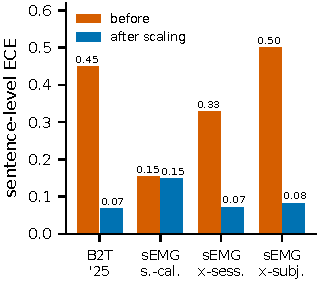
\includegraphics[width=\linewidth]{fig_ece.pdf}
    \caption{Sentence-level ECE of $\hat p_{\mathrm{top1}}$.}
    \label{fig:ece}
  \end{subfigure}\hfill
  \begin{subfigure}[t]{0.51\linewidth}
    \centering
    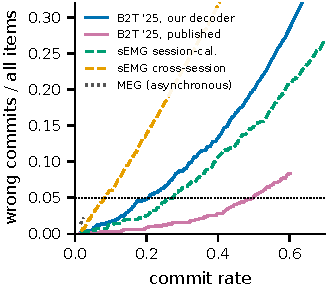
\includegraphics[width=\linewidth]{fig_risk_coverage.pdf}
    \caption{Wrong-commit rate vs commit rate.}
    \label{fig:risk}
  \end{subfigure}
  \caption{\textbf{Calibration and the commit trade-off.} (a)~Expected calibration error of the sentence confidence before and after temperature scaling (test sets). (b)~For each commit threshold on the calibrated score, the share of all test items that are committed (x) and committed wrongly (y); items blocked by the guard or other policy rules are never committed. Dotted line: $\alpha = 0.05$. The cross-subject sEMG condition is absent because no candidate passed the guard.}
  \label{fig:calib}
\end{figure}

\subsection{Null input yields no committed text}
\label{sec:res-null}
Always-commit wrote a sentence for every null input: on B2T '25 for 100\% of frame-shuffled and uniform streams, on sEMG for 100\% of frame-shuffled, zero-input and permuted-decoder streams, and on MEG for 100\% of shuffled-MEG, zero-MEG, frame-shuffled, uniform and other-sentence inputs, with fluent Spanish in 85--100\% of them (85\% on real input). The trust layer committed 0\% of null inputs on all three devices (\cref{fig:null}). On B2T '25 and sEMG this is a real test, because the same layer did commit on real input (22\% and 2.5\% of the audited items). On MEG it is not: the layer committed 0\% of real inputs as well, so the MEG audit shows that the gate stayed closed, not that it can tell null input from real input. One control it cannot pass: given the \emph{real} stream of another sentence, the trust layer on our B2T decoder committed 22\% of items, the same rate as for real input, and on sEMG it committed as often as for real input. The published-sentence gate committed 0\% in this case, because the published text did not match the other sentence's stream. A layer that sees only the stream cannot detect that the user intended a different sentence.

\begin{figure}[t]
  \centering
  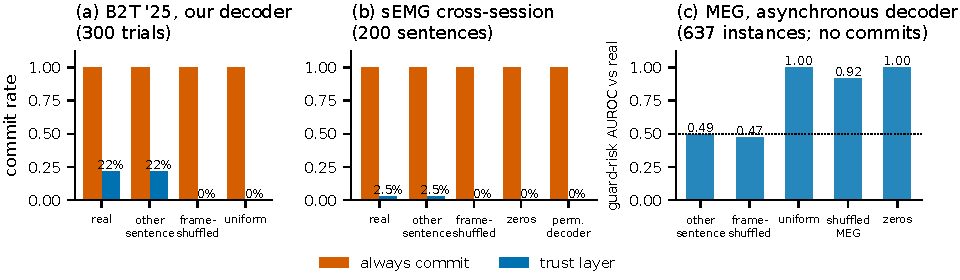
\includegraphics[width=\linewidth]{fig_null_audit.pdf}
  \caption{\textbf{Null-input audit.} Commit rate of always-commit (orange) and the trust layer (blue) on real and null inputs. (a)~B2T '25, our decoder, 300 random test trials. (b)~sEMG cross-session, 200 random test sentences. (c)~MEG, asynchronous M1-09 decoder, all 637 test instances; the trust layer also committed 0\% of real inputs, so this panel shows a closed gate, not null detection. For ``real'' and ``other sentence'', commits are a mix of right and wrong; for all other inputs any commit is wrong.}
  \label{fig:null}
\end{figure}

\subsection{Conformal risk control fixes the mean wrong-commit rate}
\label{sec:res-crc}
The plug-in policy exceeded the target on B2T '25 with our decoder (0.059 on the full test set). Over 200 random calibration/test splits with 408 calibration trials (\cref{tab:crc}, \cref{fig:crc}), CRC brought the mean test wrong-commit rate to 0.0483 (our decoder) and 0.0478 (published gate), at an \ewpm{} change of $-0.3\%$ and $+0.1\%$. LTT gave 0.0345 for both. CRC controls the mean, not every split: 41--45\% of CRC splits were above 0.05 and the 95th percentile was 0.071--0.076. LTT lowered the 95th percentile to 0.056--0.061. On MEG, where almost every possible commit is wrong, CRC still committed 2.1\% of trials (wrong-commit 0.0193; LTT 0.0214) because this is below the budget; it gained no speed (\ewpm{} 3.199 vs 3.204 for the plug-in gate, which committed nothing). Calibration splits grouped by sentence (11 of 17) or by participant (12 of 19) gave the same picture (CRC 0.0194 and 0.0201). On sEMG, with 142 calibration sentences, both methods were feasible (cross-session CRC threshold 0.204, bound 0.049) and equal to the stricter plug-in policy.

\begin{table}[t]
  \centering
  \caption{\textbf{CRC and LTT for the commit threshold} ($\alpha = 0.05$, $\delta = 0.1$, 408 calibration trials, 200 random splits). Mean over splits; p95: 95th percentile over splits. MEG: async M1-09 streams.}
  \label{tab:crc}
  \small
  \begin{adjustbox}{max width=\linewidth}\begin{tabular}{@{}llllll@{}}
    \toprule
    \textbf{Data} & \textbf{Method} & \textbf{Wrong-commit} & \textbf{p95} & \textbf{Commit rate} & \textbf{\ewpm{}} \\
    \midrule
    B2T '25, our decoder & plug-in gate & 0.0586 & 0.071 & 0.233 & 11.57 \\
     & CRC & 0.0483 & 0.071 & 0.194 & 11.53 \\
     & LTT & 0.0345 & 0.056 & 0.156 & 11.52 \\
    B2T '25, published gate & plug-in gate & 0.0441 & 0.059 & 0.471 & 18.77 \\
     & CRC & 0.0478 & 0.076 & 0.479 & 18.78 \\
     & LTT & 0.0345 & 0.061 & 0.427 & 18.70 \\
    MEG (async M1-09) & plug-in gate & 0.0000 & 0.0000 & 0.000 & 3.204 \\
     & CRC & 0.0193 & 0.0306 & 0.021 & 3.199 \\
     & LTT & 0.0214 & 0.0349 & 0.023 & 3.199 \\
    \bottomrule
  \end{tabular}\end{adjustbox}
\end{table}

\begin{figure}[t]
  \centering
  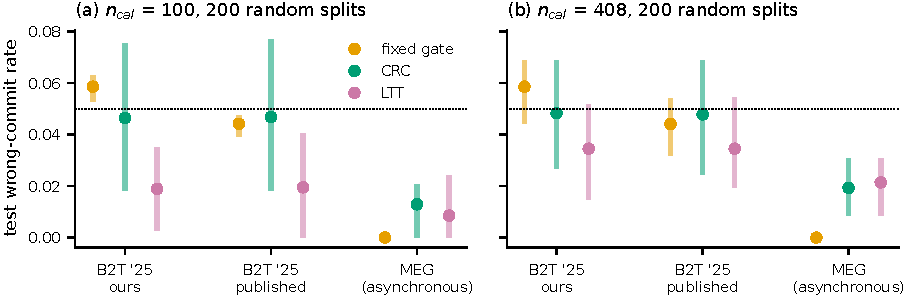
\includegraphics[width=\linewidth]{fig_crc_splits.pdf}
  \caption{\textbf{CRC controls the mean, LTT also the tail.} Test wrong-commit rate over 200 random calibration/test splits with (a)~100 and (b)~408 calibration items. Dots: mean; bars: 5th to 95th percentile. Dotted line: $\alpha = 0.05$.}
  \label{fig:crc}
\end{figure}

\subsection{Online re-calibration restores the target under drift}
\label{sec:res-drift}
CRC assumes exchangeable items. When we calibrated on the earlier half of each B2T '25 day and applied the threshold to the later half in time order, offline CRC gave 0.0625; on sEMG cross-session it gave 0.0635 (\cref{tab:drift}). The online methods brought both to 0.040--0.053 at an \ewpm{} cost of at most 0.6\%. \texttt{aci\_window} stayed below 0.05 in every drift case (0.0478 and 0.0490) and \texttt{aci} sat at the target (0.0502 and 0.0526), as its bound predicts. \Cref{fig:drift}a shows the running rate. Feedback delayed by 10 trials changed little (0.0404--0.0502 on B2T '25, our decoder). Without a calibration block (cold start over all 1,628 trials), \texttt{aci} gave 0.0442 and \texttt{aci\_window} 0.0491. No method controlled short windows: the maximum over 50-trial windows was 0.10--0.12 for all methods, as for an i.i.d.\ Bernoulli(0.05) sequence (median 0.120). When only noticed errors were fed back, \texttt{aci} gave 0.0515 on B2T '25 and 0.0635 on sEMG cross-session, because silent errors look correct to the controller.

\begin{table}[t]
  \centering
  \caption{\textbf{Wrong-commit rate under within-session drift.} Warm start on earlier data, then the later data in time order. \ewpm{} in brackets. MEG: async M1-09 streams in participant order, warm start on validation data; almost every commit is wrong. \todo{G3: CIs over days/sessions.}}
  \label{tab:drift}
  \small
  \begin{adjustbox}{max width=\linewidth}\begin{tabular}{@{}llllll@{}}
    \toprule
    \textbf{Data} & \textbf{Offline CRC} & \texttt{window} & \texttt{decay} & \texttt{aci} & \texttt{aci\_window} \\
    \midrule
    B2T '25, ours & 0.0625 (11.553) & 0.0453 (11.490) & 0.0417 (11.500) & 0.0502 (11.510) & 0.0478 (11.489) \\
    B2T '25, published & 0.0490 (18.80) & 0.0429 (18.77) & 0.0392 (18.74) & 0.0478 (18.80) & 0.0453 (18.77) \\
    sEMG cross-session & 0.0635 (4.657) & 0.0508 (4.669) & 0.0399 (4.670) & 0.0526 (4.667) & 0.0490 (4.668) \\
    MEG (async M1-09) & 0.0204 (3.198) & 0.0078 (3.201) & 0.0204 (3.198) & 0.0188 (3.200) & 0.0078 (3.201) \\
    \bottomrule
  \end{tabular}\end{adjustbox}
\end{table}

\begin{figure}[t]
  \centering
  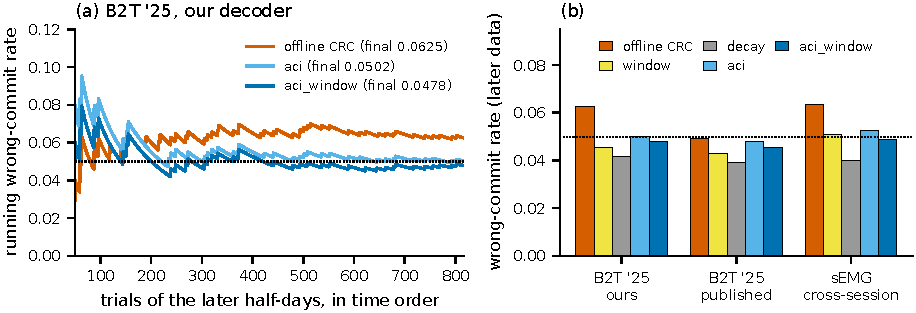
\includegraphics[width=\linewidth]{fig_drift.pdf}
  \caption{\textbf{Online re-calibration keeps the long-run rate at the target under drift.} (a)~Running wrong-commit rate over the later half-days of B2T '25 (our decoder, 816 trials, time order), recomputed from the committed per-trial items; final values equal \cref{tab:drift}. The first 50 trials are not shown. (b)~Final wrong-commit rate per method and dataset. Dotted line: $\alpha = 0.05$.}
  \label{fig:drift}
\end{figure}

\paragraph{Two CRC numbers on sEMG.} \Cref{sec:res-crc} reports a wrong-commit rate of 0.004 for CRC on sEMG cross-session, and \cref{tab:drift} reports 0.0635. Both are correct. The first combines CRC with the stricter \ewpm{}-tuned threshold ($\max(\lambda_{\mathrm{tuned}}, \hat\lambda_{\mathrm{CRC}})$); the second uses the pure CRC threshold, which exposes the drift that the stricter threshold hid.

\subsection{The ledger traces every wrong commit}
\label{sec:res-ledger}
We replayed the B2T '25 test half (816 trials) with the ledger attached, for the plug-in gate and a CRC gate. The ledger held 1,723 entries and passed verification. It found the same wrong commits as the harness: 48 of 48 (plug-in) and 39 of 39 (CRC), of which 2 and 1 were silent. Every tampering case we tried was detected: editing an entry, editing with re-hashing, deleting, reordering, and cutting the tail (with the head anchor). The cost was about 0.1\,ms and about 1.1\,kB per decision. \Cref{fig:audit} shows one entry of the audit report: most wrong commits were one-word errors.

\subsection{Ablations}
\label{sec:res-ablation}
On B2T '25, removing calibration raised the wrong-commit rate from 0.059 to 0.071 (\ewpm{} 11.57 vs 11.55), and removing the guard lowered it to 0.036 (\ewpm{} 11.51): the guard did not help on this device. On sEMG session-calibrated, removing calibration raised the wrong-commit rate from 0.004 to 0.045 and \ewpm{} from 8.02 to 8.15. \todo{G5: one unified ablation table over the three devices (calibration, guard, conformal sets, \act{offer\_words}, CRC on/off), same seeds.}

\begin{figure}[t]
  \centering
  \fbox{\begin{minipage}{0.94\linewidth}\footnotesize\raggedright
  \textbf{Wrong commit} \texttt{dec-000041-ed60b4bd} (entry 44, hash \texttt{8cf2c6c67053b185...})\\
  Committed: ``who you never expect to when''\\
  Correction (oracle ground truth, hash-linked): ``who you never expect to win''; 2 character edits, 1 word edit\\
  Scores: $\hat p_{\mathrm{top1}}$ 0.5814, set size 3, guard risk 0.2857; reason: $\hat p_{\mathrm{top1}} \ge 0.50$\\
  Input: stream \texttt{1b4b60e8e4950710...}, frames [0, 335], item \texttt{b2t25-test-trial-196}\\
  Decoder: published online RNN + our phoneme-to-word decoder; LM: Tatoeba character 6-gram + word unigram + CMUdict; adapter \texttt{fidetype.adapters.b2t25}\\
  Calibration \texttt{cal-692fb52a73417552}: $T_f$ 3.7809, $T_s$ 4.5551, fit set: first half of each day (812 trials)\\
  Policy \texttt{pol-2eaa4ff51919527a}: commit threshold 0.5, maximum guard risk 0.5, offer size 2
  \end{minipage}}
  \caption{\textbf{One entry of the provenance audit report} (B2T '25 replay, plug-in gate; public CC0 cue sentence). Each wrong commit is traced to the exact stream segment and to the decoder, LM, calibration and policy versions that produced it. Hashes are shortened.}
  \label{fig:audit}
\end{figure}

\section{Discussion}
\label{sec:discussion}

\paragraph{The layer is a safety mechanism, tested non-trivially on one person.} All non-trivial evidence for the commit decision comes from one intracortical participant in a copy task; sEMG sentences were composed from isolated presses, and MEG was a negative control. On that participant, a stream-only rule with a high-probability guarantee kept the wrong-commit rate at or below 5\% in 92\% (our decoder) and 98\% (published decoder) of repeated deployments, at a mean of 3\%, and it stayed faster than always offering in every deployment, by 0.11 and 0.51 \ewpm{}. Whether it beat always committing depended on unmeasured user costs, and on weaker decoders a gaze keyboard with simple word completion was faster still, so we make no general speed claim. On sEMG and MEG the layer reduced to always offering, the correct behaviour for decoders whose top sentence was rarely right; it cannot create information that the decoder lacks.

\paragraph{Which guarantee to deploy.} CRC met its target as a mean over deployments, exactly as it promises, but a third or more of single deployments exceeded $\alpha$; so did the plug-in rule. A user lives in one deployment, so the per-deployment (high-probability) guarantee of LTT is the relevant one, and the max rule costs almost nothing (0.01--0.04 \ewpm{} against CRC with the max rule). Each guarantee should be stated with its assumptions, its target, its unit of exchangeability and the measured silent-error rate (\cref{app:guarantees}). On MEG the unit is the sentence, and no guarantee for new sentences is possible with 17 test sentences.

\paragraph{Who sets $\alpha$, and for which error.} The marginal wrong-commit rate is the budget of harm per sentence attempted; the error among commits is what a user sees in committed text. With current decoders the two diverge: one in five commits of the guaranteed rule on our decoder was wrong, and a user who sees this will learn to check every commit, which turns commits into offers. A guaranteed error among commits of 10\% was reachable only for the published decoder, and only in about a third of deployments with 400 calibration trials. With a few hundred calibration sentences, a certified ``one wrong committed sentence in ten'' is possible only for the strongest decoder; the joint rule (marginal $\le \alpha$ and selective $\le \beta$) is the one to recommend. The targets should come from users. Potential BCI users with ALS or spinal cord injury asked for at least 90\% accuracy \citep{huggins2011als,huggins2015sci}, which suggests $\beta \le 0.10$ rather than a marginal target alone. The choice should be made by the user with their clinician and communication partners, explained in these terms (``at most one in ten sentences that the system sends by itself is wrong''), and it may differ by context: a casual conversation tolerates more than a medical decision or a message to a stranger. AAC users care about text that is sent in their name \citep{valencia2023aac,kane2017avuncular}, and our exact-match loss treats a harmless near miss (``who you never expect to when'') like a meaning-changing error (``I want to stop'' vs ``I want to start''). A loss weighted by semantic severity, scored by users, is the natural next target.

\paragraph{Calibration data must play no other role.} Calibrating on data that had also fitted the pipeline raised the mean CRC wrong-commit rate on our decoder above $\alpha$, but not on the published gate or sEMG, and the effect was a quarter of one deployment's spread; drift, reuse and split variation cannot be separated on one fixed split. In data-scarce BCI pipelines this mistake is easy. Papers should state which data fitted each stage and repeat the fit/calibration assignment before they claim a shift or a guarantee.

\paragraph{Strong decoders still need a gate.} The published Brain-to-Text '25 decoder has a WER of 0.043, yet 19\% of its sentences were wrong. Gating its text by agreement with the neural evidence kept 96\% of the always-commit \ewpm{} under the main simulated user and reduced wrong commits to 4.4\% (plug-in) and 3.1\% (guaranteed rule, mean over deployments), using only the stream, the published text and a light reference decoder. This is what a vendor-neutral stream interface enables; on sEMG, in-session decoder data gave 71\% higher \ewpm{} than another day's data (8.02 vs 4.68), so adaptation, not the layer, makes a weak decoder fast. The trust layer took a median of 0.18--0.30\,ms per decision on one CPU thread (95th percentile at most 1.1\,ms), against 45--232\,ms for the beam-search decoders, so it adds no meaningful latency.

\paragraph{A frozen configuration for a confirmatory test.} Every revision of this paper looked at the same Brain-to-Text '25 test half, so all results here are exploratory. For a confirmatory test on data we have not used (a second participant, or held-out sessions), we fix the configuration now: frame and sentence temperatures, plain calibrated threshold without the guard, policy grid of \cref{tab:settings} fitted on fit-A, LTT with the max rule on a disjoint calibration set, $\alpha = 0.05$, $\delta = 0.1$, and the joint selective constraint with $\beta = 0.10$; primary outcomes are the wrong-commit rate and the error among commits, with their share of deployments above target. This configuration is tagged \code{paper1-v3-frozen-config} in the repository.

\section{Limitations}
\label{sec:limitations}

\begin{enumerate}[leftmargin=*,itemsep=0pt]
  \item \textbf{One implant participant} in a copy task, with online logits we cannot re-run, is the only non-trivial test of the commit decision; our intervals cover days, not people.
  \item \textbf{Composed sEMG sentences}: isolated presses with oracle timing, recurring presses, and test sentences from the LM's corpus (295 of 551 have a near variant in the LM text; removing them changed trust \ewpm{} by at most $-0.04$, \cref{app:leakage}). \textbf{MEG is a negative control}: 17 unique test sentences, and a decoder that uses key times as training labels and keyboard-log sentence bounds.
  \item \textbf{No live users.} Only two user costs are measured, in one gaze-typing user; the miss probability is unmeasured; the MEG and sEMG populations do not match; speed rankings change across plausible variants; the word-completion baseline uses only a unigram. A user study needs ethics approval.
  \item \textbf{One seed and one split per run.} MEG decoder seeds 1 and 2 are still training; sEMG seeds, repeated Brain-to-Text '25 fit/test assignments and a k-fold over MEG sentences were not run. The two deployment splits moved offline CRC from 0.0245 to 0.0600. Trial order is file order (no time stamps), so ``no detectable within-day shift'' holds for this order only.
  \item \textbf{Scope of the guarantees.} They are marginal or long-run (43--46\% of single CRC splits exceeded 0.05), count only observed errors, and do not bound the error among commits. Stream-only gating cannot detect intent mismatch; the loss is exact match (we did not test a tolerant loss); the audit log is tamper-evident, not tamper-proof.
\end{enumerate}

\section{Conclusion}
\label{sec:conclusion}

A trust layer that reads only a per-frame output stream can decide whether a neural text-entry decoder commits, offers or abstains under a stated bound on the wrong-commit rate. On one intracortical participant it turned frequent wrong commits into rare ones at little or no speed cost relative to always offering, while one committed sentence in four (our decoder) or eleven (published decoder) was still wrong; on composed sEMG sentences and a weak MEG decoder it almost never or never committed. With calibration data that played no other role, conformal calibration met its target on later data up to sampling variation; an apparent drift failure was data reuse. Next steps are a gaze-typing user study, a controller for the error among commits, and the public benchmark that the release starts.

\section{Ethics, data and code availability}
\label{sec:ethics}
\label{sec:availability}

This study uses only public, de-identified datasets; no new data were collected and no experiment with human participants was run, so no new ethics approval was required. The intracortical data come from a participant in the BrainGate2 pilot clinical trial \citep{card2024accurate}; we use only the released copy-task logits and sentences and did not attempt re-identification. \todo{author decision: final wording and the venue's policy on secondary use of public clinical-trial data.} No raw recordings or participant data are redistributed; \cref{tab:licences} lists all datasets and licences. The \nts{} specification, conformance suite, reference implementation, benchmark scorer and all experiment scripts are at \url{https://github.com/zhangzibo/fidetype} (Apache-2.0), without weights trained on SpanishBCBL or copied Brain2Qwerty code; every table and figure is generated from committed result files. \todo{tag the paper commit and archive it (e.g.\ Zenodo DOI).} Decoders were trained on one AMD RX 7800 XT GPU; trust-layer runs use a CPU. \todo{report trust-layer run time per decision.}


\section*{Acknowledgements}
\todo{funding.} AI coding and writing assistants were used under human review; all numbers come from committed scripts and result files. \todo{author: final AI-assistance wording.}

\bibliographystyle{unsrtnat}
\bibliography{refs}

\appendix
\section{Notation}
\label{app:notation}

\begin{table}[!htb]
  \centering
  \caption{\textbf{Notation.}}
  \label{tab:notation}
  \small
  \begin{tabular}{@{}ll@{\qquad}ll@{}}
    \toprule
    \textbf{Symbol} & \textbf{Meaning} & \textbf{Symbol} & \textbf{Meaning} \\
    \midrule
    $F_i$ & frames in the stream of item $i$ & $\lambda$ & commit threshold on $s_i$ \\
    $V$ & vocabulary size of the stream & $s_i$ & commit score of item $i$ (\cref{sec:crc}) \\
    $K$ & size of the candidate list ($K = 10$) & $n$ & number of calibration items \\
    $k$ & number of offered candidates & $T$ & number of items in an online sequence \\
    $\tau_f$, $\tau_s$ & frame and sentence temperatures & $\eta$, $\gamma$ & step sizes of the online controllers \\
    $c_i$, $f_i$ & commit loss, non-commit loss & $\alpha$, $\delta$ & target risk, LTT failure probability \\
    \bottomrule
  \end{tabular}
\end{table}

\section{User model parameters}
\label{app:user}

\Cref{tab:user} lists the parameters of the simulated gaze-typing user (word model: the user fixes single words). Only the fallback typing speed and the per-slot scan-and-select time are matched to measurements of one eye-gaze user with ALS \citep{cai2024gaze}; all other values are assumptions. The baseline ``gaze typing only'' uses the fallback speed alone.

\begin{table}[!htb]
  \centering
  \caption{\textbf{Simulated-user parameters.}}
  \label{tab:user}
  \small
  \begin{adjustbox}{max width=\linewidth}\begin{tabular}{@{}lll@{}}
    \toprule
    \textbf{Parameter} & \textbf{Value} & \textbf{Basis} \\
    \midrule
    Fallback (gaze keyboard) speed & 20 characters/min & measured, eye-gaze user LP1 \citep{cai2024gaze} \\
    Scan and select one of $k$ word alternatives & $1.0 + 1.0\log_2(k+1) + 1.5$\,s (4.5\,s for $k = 3$) & sum matched to 4.7\,s \citep{cai2024gaze} \\
    Select one of $k$ offered sentences & $1.0 + 0.5\log_2(k+1)$\,s & assumption \\
    Reading time & 0.3\,s per word, 0.5\,s per candidate & assumption \\
    Navigate to and delete a wrong word & 3.0\,s (2 selections) & assumption \\
    Miss probability of a wrong, unmarked word (commit, \act{offer\_words}) & 0.05 & assumption (no measurement) \\
    Errors in offered candidates & always seen & assumption \\
    Full retype overhead & 1.5\,s; chosen when cheaper than fixing words & assumption (rational user) \\
    Abstain overhead & 0.5\,s, then fallback typing & assumption \\
    Neural input speed, MEG / B2T '25 / sEMG & 152 / 159.3 / 75.8 characters/min & device setting \\
    \bottomrule
  \end{tabular}\end{adjustbox}
\end{table}

\section{Per-device settings}
\label{app:settings}

\Cref{tab:settings} lists the parameters that the shared implementation fitted or used per device. The policy grid and all decoder settings are in the experiment configurations in the repository.

\begin{table}[!htb]
  \centering
  \caption{\textbf{Per-device settings of the shared trust-layer implementation.} Fitted on each device's fit data (MEG: validation set). $\tau_s = 20.0$ is the upper end of the search interval. Max.\ guard risk: largest guard risk that still allows a commit.}
  \label{tab:settings}
  \small
  \begin{adjustbox}{max width=\linewidth}\begin{tabular}{@{}lllll@{}}
    \toprule
    & \textbf{MEG} & \textbf{B2T '25, ours} & \textbf{B2T '25, published gate} & \textbf{sEMG (cal.\ / x-sess.\ / x-subj.)} \\
    \midrule
    Frame temperature $\tau_f$ & 3.30 & 3.78 & 3.78 & 1.25 / 1.78 / 2.17 \\
    Sentence temperature $\tau_s$ & 20.0 & 4.56 & 1.72 & 2.42 / 5.42 / 20.0 \\
    LM weight (beam) & 0.5 & 1.0 (word LM; edit penalty 12, word bonus 3) & as ours & 1.0 / 1.0 / 1.5 \\
    Candidate list $K$ & 10 & 10 & published sentence + our 10 (bonus +2.0) & 10 \\
    Plug-in commit threshold & 0.5 & 0.5 & 0.7 & 0.7 / 0.3 / 0.3 \\
    Max.\ guard risk for commit & 0.3 & 0.5 & 0.5 & 1.0 / 1.0 / 0.1 \\
    Offer size $k$ & 1 & 2 & 1 & 2 / 2 / 1 \\
    Fallback after offer & offer & offer & offer & offer \\
    Guard & \multicolumn{4}{l}{low-evidence threshold 0.5; consistency over the top 5; risk $=\max$(low evidence, 1 $-$ consistency), weights 1} \\
    Adapter (lines of Python) & 148 & 412 & 412 & 568 \\
    \bottomrule
  \end{tabular}\end{adjustbox}
\end{table}

\section{MEG decoder, leakage checks and sensitivity}
\label{app:meg}

The asynchronous MEG decoder is a convolutional front end (320 channels) followed by 4 Conformer layers of width 256 \citep{gulati2020conformer}, trained with CTC \citep{graves2006ctc} and a keystroke auxiliary loss that uses key times as training labels (key pretraining, then CTC training on all 80 recording blocks). At inference, the forward pass takes the MEG segment, its length and the participant index; it has no key input. \Cref{tab:async} compares the inference inputs with the published asynchronous decoder.

\begin{table}[!htb]
  \centering
  \caption{\textbf{Asynchronous setting: our decoder vs Brain2Qwerty v2.}}
  \label{tab:async}
  \small
  \begin{tabular}{@{}lll@{}}
    \toprule
    \textbf{Input at inference} & \textbf{Ours} & \textbf{v2 async \citep{zhang2026brain2qwertyv2}} \\
    \midrule
    MEG of the sentence segment & yes & yes \\
    Segment start & first key $-$ 0.4\,s & first key $-$ 400\,ms \\
    Segment end & last key press + 0.5\,s & last key release + 400--500\,ms \\
    Per-key times or key count & no & no \\
    Participant index & yes & yes \\
    Key times as training labels & yes (auxiliary loss) & no \\
    \bottomrule
  \end{tabular}
\end{table}

\paragraph{Leakage checks.} The split is by a hash of the sentence text, and no test sentence occurs in the LM training text. A test sentence is ``close'' if a training sentence is within CER 0.25; 6 of the 17 test sentences are close. Without them, the CER was 0.519 (greedy) and 0.492 (beam).

\paragraph{Synchronous control decoder.} A synchronous decoder with oracle key times (greedy CER 0.508, beam + LM 0.447; harness top-1 CER 0.451) gave the same trust results as the asynchronous decoder: always commit 2.714, trust 3.229 and gaze typing 3.155 \ewpm{}, trust minus gaze \ci{-0.02}{+0.18} over sentences and \ci{-0.07}{+0.26} two-way. Over trials, this difference excluded 0 (\ci{+0.03}{+0.12}): trial-level intervals make the MEG result look like a gain, and sentence-level intervals do not. Both decoders take the sentence bounds from the keyboard log, so neither is a free-running decoder. \todo{R1: k-fold over sentence hashes to increase the number of unique MEG test sentences.}

\paragraph{User-model sensitivity on MEG.} \Cref{tab:megsens} refits the policy under each user-model variant (asynchronous decoder). The trust layer equals always offering in every variant. The advantage over always commit depends on the miss probability, and the comparison with gaze typing reverses with a faster fallback or slower selection. \todo{R1: the same grid on B2T '25 and sEMG, with the policy ranking and a misspecified-user evaluation.}

\begin{table}[!htb]
  \centering
  \caption{\textbf{User-model sensitivity, MEG (asynchronous decoder; policy refitted per variant).} \ewpm{}; CIs over the 17 unique sentences and over the 19 participants.}
  \label{tab:megsens}
  \small
  \begin{adjustbox}{max width=\linewidth}\begin{tabular}{@{}lllllll@{}}
    \toprule
    \textbf{Variant} & \textbf{Always commit} & \textbf{Trust} & \textbf{Gaze only} & \textbf{Trust $-$ gaze [sent.]} & \textbf{\{part.\}} \\
    \midrule
    Main (miss 0.05, fallback 20 cpm) & 2.58 & 3.20 & 3.15 & \ci{-0.04}{+0.15} & \{$-$0.07, +0.22\} \\
    Fallback 40 characters/min & 4.31 & 5.15 & 6.31 & \ci{-1.29}{-1.01} & \{$-$1.31, $-$0.95\} \\
    Miss probability 0 & 3.24 & 3.20 & 3.15 & \ci{-0.04}{+0.15} & \{$-$0.08, +0.22\} \\
    Miss probability 0.2 & 1.24 & 3.20 & 3.15 & \ci{-0.04}{+0.15} & \{$-$0.08, +0.22\} \\
    Selection, scan and navigation $\times 2$ & 2.54 & 3.00 & 3.15 & \ci{-0.23}{-0.08} & \{$-$0.26, $-$0.02\} \\
    No full retype & 2.54 & 3.18 & 3.15 & \ci{-0.06}{+0.13} & \{$-$0.10, +0.21\} \\
    \bottomrule
  \end{tabular}\end{adjustbox}
\end{table}

\section{Format details and audit log}
\label{app:format}

\paragraph{Serialisations and conformance.} The reference serialisations of \nts{} are an NPZ file and a JSON Lines streaming form. A conformance suite runs 60 checks, each tied to a specification clause, and reports one of three cumulative levels: \emph{core} (a consumer must accept the stream), \emph{trust-ready} (modality, causality, calibration state and language are declared) and \emph{provenance} (stream id, decoder name, version and weights hash). It ships 52 golden test vectors (32 NPZ, 20 JSON Lines); the reference consumer passes 52 of 52. On synthetic inputs, our MEG and sEMG adapters reach the provenance level and the intracortical adapter reaches trust-ready, because the published online decoder has no weights file to hash. Writing the suite found five bugs in our own producers and ten ambiguities in the specification text, now listed as open questions.

\paragraph{Audit log.} Each decision can be appended to a JSON Lines log. Context entries are content-addressed (their id is the SHA-256 of the context) and hold the adapter, decoder (name, version, weights hash, training data and licence), LM, calibration (temperatures, risk-control method, $\alpha$, $\delta$, threshold, $n$) and policy versions; decision entries hold the action, scores, a hash of the stream and its frame range; correction entries link to the decision they correct. Each entry stores the hash of the previous entry and its own SHA-256 over the canonical JSON, so any edit, deletion or reordering breaks the chain; a separately stored head anchor detects truncation. The log stores no raw signals (numeric arrays longer than 64 values are rejected), stores text as a keyed hash by default, and pseudonymises subject and session ids. It is tamper-evident, not tamper-proof: there is no signature in v0.

\paragraph{Replay.} We replayed the Brain-to-Text '25 test half (816 trials) with the log attached, for the plug-in gate and a CRC gate. The log held 1,723 entries and passed verification. It recorded the same wrong commits as the harness: 48 of 48 (plug-in) and 39 of 39 (CRC), of which 2 and 1 were silent. This is a consistency check of the replay: the corrections come from the known cue sentences, and in live use silent errors would be missing from the log. Every tampering case we tried was detected: editing an entry, editing with re-hashing, deleting, reordering, and cutting the tail (with the head anchor). The cost was about 0.1\,ms and about 1.1\,kB per decision. \Cref{fig:audit} shows one entry of the audit report.

\begin{figure}[!htb]
  \centering
  \fbox{\begin{minipage}{0.94\linewidth}\footnotesize\raggedright
  \textbf{Wrong commit} \texttt{dec-000041-ed60b4bd} (entry 44, hash \texttt{8cf2c6c67053b185...})\\
  Committed: ``who you never expect to when''\\
  Correction (known cue sentence, hash-linked): ``who you never expect to win''; 2 character edits, 1 word edit\\
  Scores: $\hat p_{\mathrm{top1}}$ 0.5814, set size 3, guard risk 0.2857; reason: $\hat p_{\mathrm{top1}} \ge 0.50$\\
  Input: stream \texttt{1b4b60e8e4950710...}, frames [0, 335], item \texttt{b2t25-test-trial-196}\\
  Decoder: published online RNN + our phoneme-to-word decoder; LM: Tatoeba character 6-gram + word unigram + CMUdict; adapter \texttt{fidetype.adapters.b2t25}\\
  Calibration \texttt{cal-692fb52a73417552}: $\tau_f$ 3.7809, $\tau_s$ 4.5551, fit set: first half of each day (812 trials)\\
  Policy \texttt{pol-2eaa4ff51919527a}: commit threshold 0.5, maximum guard risk 0.5, offer size 2
  \end{minipage}}
  \caption{\textbf{One entry of the audit report} (B2T '25 replay, plug-in gate; public CC0 cue sentence). Each wrong commit is traced to the exact stream segment and to the decoder, LM, calibration and policy versions that produced it. Hashes are shortened.}
  \label{fig:audit}
\end{figure}

\section{Online re-calibration methods}
\label{app:online}

\begin{table}[!htb]
  \centering
  \caption{\textbf{Online re-calibration methods for the commit threshold.} $L_t$: realised loss of item $t$; $T$: number of items in the sequence; $d$: feedback delay in items. The two \texttt{aci} variants bound the long-run average of the \emph{observed} losses for any sequence of items, without exchangeability; \texttt{window} and \texttt{decay} have no guarantee under shift.}
  \label{tab:online}
  \small
  \begin{adjustbox}{max width=\linewidth}\begin{tabular}{@{}llll@{}}
    \toprule
    \textbf{Method} & \textbf{Update} & \textbf{Guarantee} & \textbf{Feedback} \\
    \midrule
    \texttt{window} & CRC on the last $N = 200$ items with known truth & none under shift$^{a}$ & full \\
    \texttt{decay} & weighted CRC on all past items, weights $\rho^{\text{age}}$, $\rho = 0.99$ & none under shift$^{a}$ & full \\
    \texttt{aci} & $\lambda_{t+1} = \max(0, \lambda_t + \eta(L_t - \alpha))$, $\eta = 0.05$ & $\frac1T\sum_t L_t \le \alpha + \frac{\lambda_{T+1} - \lambda_1}{\eta T}$ $^{b}$ & realised only \\
    \texttt{aci\_window} & window CRC at level $\alpha_t$; $\alpha_{t+1} = \min(2\alpha, \alpha_t + \gamma(\alpha - L_t))$, $\gamma = 0.005$ & $\frac1T\sum_t L_t \le \alpha + \frac{\alpha_1 - \alpha_{T+1}}{\gamma T}$ $^{c}$ & full + realised \\
    \bottomrule
  \end{tabular}\end{adjustbox}
  \begin{minipage}{\linewidth}\footnotesize\smallskip
  $^{a}$ The weighted-CRC bound $\alpha + \sum_i \tilde w_i\, d_{\mathrm{TV}}(Z, Z^{(i)})$ \citep{barber2023beyond,farinhas2024nonexch} cannot be computed. Items whose truth is unknown are left out of the window, which can bias it. \\
  $^{b}$ The right-hand side is a certificate computed after the fact. It is bounded in advance only if $\lambda_t$ stays bounded, which holds for scores $\le 1$ and $f \equiv 0$; then $\frac1T\sum_t L_t \le \alpha + \frac{1 - \lambda_1 + \eta(1+d)}{\eta T}$, which is 0.064 for $T = 816$, $\eta = 0.05$, $d = 0$ and the B2T '25 start threshold. \\
  $^{c}$ The upper clip at $2\alpha$ only lowers $\alpha_t$, so the bound stays valid. $\alpha_t$ stays bounded below because below the CRC feasibility level ($\approx 1/(N+1)$) nothing is committed and $\alpha_t$ rises. \\
  All bounds count only the losses that the controller observes. Items whose feedback has not arrived are skipped; in our runs all feedback arrived after the delay, except in the ``noticed errors only'' runs, where a silent error is fed back as a correct commit.
  \end{minipage}
\end{table}

\section{Additional risk-control results}
\label{app:more}

\Cref{fig:crc} shows the spread of the test wrong-commit rate over the 200 random calibration/test splits for 100 and 408 calibration items. For \texttt{aci} on Brain-to-Text '25 (our decoder), step sizes $\eta$ of 0.01, 0.02, 0.05, 0.1 and 0.2 gave wrong-commit rates of 0.0527, 0.0515, 0.0502, 0.0502 and 0.0502, with a-priori bounds of 0.114, 0.083, 0.064, 0.058 and 0.054. On sEMG session-calibrated, pure offline CRC was below the target (0.0417), and the online methods gave 0.0454--0.0490; on sEMG cross-subject nothing could be committed.

\begin{figure}[!htb]
  \centering
  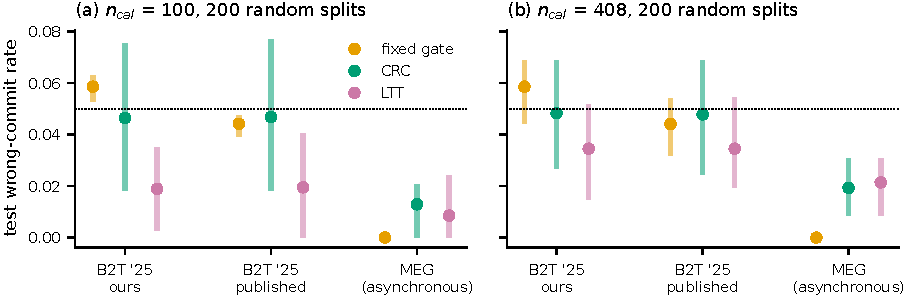
\includegraphics[width=\linewidth]{fig_crc_splits.pdf}
  \caption{\textbf{CRC bounds the mean over splits; LTT bounds the calibration-conditional risk with probability $1 - \delta$.} Test wrong-commit rate over 200 random calibration/test splits with (a)~100 and (b)~408 calibration items. Dots: mean; bars: 5th to 90th percentile (the 90th percentile matches $\delta = 0.1$). Dotted line: $\alpha = 0.05$. A test rate above $\alpha$ in a single split is not a violation of either guarantee.}
  \label{fig:crc}
\end{figure}


\end{document}
